%!TEX root = ../main.tex
\appendix
\appendixpageoff
\section{Appendix A. Skewed Student-\textit{t} distribution} \label{App:AppendixA}
In line with stylized facts on financial return series, the factor strategies exhibit fat tails and skewness - features that are poorly represented by the normal Gaussian. Our univariate estimations as well as our copula builds on the~\textcite{Hansen1994} skewed Student-\textit{t} distribution. The skewed Student-\textit{t} distribution is, more generally, nested in the generalized hyperbolic distribution~\autocite{McNeilFreyEmbrecht2005}.

The random vector X is distributed multivariate generalized hyperbolic if
\begin{align}
    X \sim \mu + \sqrt{W} A Z + \gamma W
\end{align}
where $\mu$ is the location vector, $\gamma$ is the skewness vector, $R = A A^\top$ is the dispersion matrix, $W$ follows a generalized inverse-gamma distribution $W \sim GIG(\lambda, \chi, \psi)$ and Z is multivariate normal $Z \sim N(\mu^N, R)$, with $W, Z$ independent. The skewed Student-\textit{t} is nested with parameters
\begin{align}
    \lambda = \frac{\nu}{-2} && \chi = \nu - 2 && \psi = 0
\end{align}
where $\nu$ is the degree of freedom. Furthermore
\begin{align}
    \mathbb{E}[X] &= \mu + \mathbb{E}[W] \gamma \\
    Var[X] &= \mathbb{E}[Cov(X|W)] + Cov(\mathbb{E}[X|W]) \\
    &= Var(W) \gamma \gamma^\top + \mathbb{E}[W] R \nonumber
\end{align}
These moments describe the link between the copula correlation matrix $R$ and the skewed Student-\textit{t} distribution's dispersion matrix $R$. Covariances are finite when $\nu > 4$. The multivariate density function is given by
\begin{align} \label{eq:dskewt}
    f_X(x) &= \frac{(\nu - 2)^\frac{\nu}{2} (\gamma^\top R^{-1} \gamma)^{\frac{\nu+d}{2}}}{(2 \pi)^{\frac{d}{2}} |R|^\frac{1}{2} \Gamma (\frac{\nu}{2}) 2^{\frac{\nu}{2} - 1}} \cdot \frac{K_{\frac{\nu + d}{2}} ( \sqrt{(\nu - 2 + Q(x)) \gamma^\top R^{-1} \gamma}) e^{(x-\mu)^\top R^{-1} \gamma} )}{( \sqrt{(\nu - 2 + Q(x)) \gamma^\top R^{-1} \gamma})^{\frac{\nu + d}{2}}}
\end{align}
where $K(\cdot)$ is the modified Bessel function of the second kind, $Q(x) = (x-\mu)^\top R^{-1} (x-\mu)$, $d$ is the length of $x$, and $\Gamma$ is the gamma distribution density.

\newpage
\section{Appendix B. ARMA-GARCH modeling of marginal distributions} \label{App:AppendixB}

By examining marginal factor strategy returns (see \autoref{App:AppendixF}), we find evidence of non-normality, autocorrelation, volatility clustering and leverage effects, in line with stylized factors on financial return series (\textcite{Bollerslev1986}, \textcite{Black1976}, \textcite{glosten1993relation}). An ARMA-GARCH model allows us to filter away such marginal asymmetries, while leaving any multivariate asymmetry to the copula specification. The goal of this GARCH model is not to have high predictive power of asset return series, but to sanitize the data to be used in multivariate analysis. We focus on parsimonious models with few lags, but enough flexibility to capture salient features of the summary plots of the marginal series, such as volatility clustering and leverage effect.

The selection process is as follows: for each factor strategy, ARMA-GJR-GARCH models are estimated with different ARMA lag orders (up to 3,3) and a fixed GJR-GARCH order of (1,1). We then compute the Bayesian Information Criterion (BIC, \textcite{Schwarz1978}) for each specification, and for each factor select the model with the lowest BIC as the primary candidate. The primary candidate specification is then checked for remaining serial correlation and ARCH effects in residuals, using the weighted portmanteau tests of \textcite{FisherGallagher2012}. All of the primary candidate models pass the diagnostic tests (see \autoref{App:AppendixE}), and additional diagnostics plots are available (see \autoref{App:AppendixG}). We use the GJR-GARCH model with ARMA mean equation
\begin{align}
    r_t &= \mu + \sum^p \phi_p r_{t-p} + \sum^q \theta_q \epsilon_{t-q} + \epsilon_{t}  \\
    \sigma_{t}^2 &= \omega + (a + \eta I_{t-1}) \epsilon_{t-1}^2 + b \sigma^2_{t-1}
\end{align}
which is estimted using maximum likelihood for each of the factor return series. The innovations $\epsilon_{i,t}$ are assumed to be distributed skewed Student-\textit{t} with skewness $\zeta$ and degree of freedom $\varrho$.

Using conditional one-step-ahead forecasts of log return and standard deviation from the ARMA-GARCH model, we can compute standardized GARCH residuals
\begin{align}
    \epsilon^*_{i,t} = \frac{\epsilon_{i,t} - E_{t-1}[\epsilon{i,t}]}{E_{t-1}[\sigma(\epsilon{i,t})]}
\end{align}
which are subsequently transformed into uniform residuals using the inverse of the skewed Student-\textit{t} distribution (\autoref{eq:dskewt}). The uniform series $\{u_i\}$ are then employed in the copula estimation.
\begin{align}
    u_{i,t} = t^{-1}_{\zeta, \varrho}(\epsilon^*_{i,t})
\end{align}

\newpage
\section{Appendix C. Stationary bootstrap of copula parameter standard errors} \label{App:AppendixC}
We rely on the multi-step maximum likelihood estimation of the copula model, which takes the standardized residuals of marginal distributions as given in the second step. The first estimation step introduces parameter uncertainty that is not taken into account by the conventional standard errors of the second estimation.\footnote{Here, our model deviates from~\textcite{ChristoffersenLanglois2013}, who use a semi-parametric model that uses the empirical density function, and find standard errors using the analytical approach in~\textcite{ChenFan2006}. However, those errors are not valid in a time-varying copula context, as the estimation of means and variances impact the asymptotic distributions of copula parameters~\autocite{Remillard2010}.} We use the stationary block bootstrap method of \textcite{PolitisRomano1994} with a block length of 45 weeks (approx. 1 year of data) to find reliable standard errors for copula parameters. The procedure is theoretically supported by \textcite{GonclavesWhite2004} and implemented as follows:
\begin{enumerate}[(i)]
    \item Generate a block bootstrap version of the original weekly return data
    \item Estimate the ARMA-GJR-GARCH models and calculate standardized residuals
    \item Transform standardized residuals to uniform and estimate the copula model
    \item Collect the copula parameters $\Theta_i$
    \item Repeat (i)-(iv) N times to get $\{\Theta_i\}^{N}_{i=1}$
    \item Use the standard errors from the empirical distribution of $\{\Theta_i\}^{N}_{i=1}$
\end{enumerate}

\newpage
\section{Appendix D. Copula correlation matrix estimation with \textit{c}DCC dynamics} \label{App:AppendixD}
This is a step-by-step description of the procedure used to find the copula correlation matrix $\{\hat{R_t}\}$ in the \textit{c}DCC case, and has been adapted from \textcite{Aielli2013}.
\begin{enumerate}[(i)]
    \item Re-standardize uniform residuals from univariate ARMA-GJR-GARCH models $\{u_{i}\}$ using the inverse skewed Student-\textit{t} distribution with copula parameters $\nu, \gamma$,  and scale to zero mean and unit variance using the conditional mean and standard deviation\footnote{Unless the copula is normal, the re-standardized residuals $\{\varepsilon^c_i\}$ will not have zero mean and unit variance, which is required for the estimation of the sample correlation matrix $\hat{S}$.}
    \begin{align}
        \varepsilon^c_{i,t} = t^{-1}_{\gamma, \nu}(u_{i,t})
    \end{align}
    \begin{align}
        \varepsilon_{i,t} = \frac{\varepsilon^c_{i, t} - E_{t-1}[\varepsilon^c_{i,t}]}{E_{t-1}[\sigma(\varepsilon^c_{i,t})]}
    \end{align}
    \item Compute the diagonal elements in $Q_t$ over time recursively, initializing with unit diagonal, and using Q-residuals $\{z_i\}$
    \begin{align}
        \intertext{Utilizing that $\S_{ii} = 1$ (for any correlation matrix), the process for diagonal elements of Q simplifies to}
        q_{ii, t} &= (1 - \alpha - \beta) + \alpha z_{t-1} z_{t-1}^\top + \beta q_{ii, t-1}
        \intertext{where residuals $\{z_{i}\}$ are initialized at zero and then calculated as}
        z_{i, t} &= \varepsilon_{i, t} \sqrt{q_{ii, t}}
    \end{align}
    \item \label{cdcc:momS} Use Q-standardized residuals $\{z_{i}\}$ to calculate a copula sample correlation matrix
    \begin{align}
        \hat{S} = \frac{1}{T} \sum_{t=1}^{T} z_{t} z_{t}^\top
    \end{align}
    \item Calculate off-diagonal elements of the Q matrix using the copula sample correlation matrix $\hat{S}$ as the long-term correlation matrix in the \textit{c}DCC specification
    \begin{align}
        \hat{Q_t} = (1 - \alpha - \beta) \hat{S} + \alpha z_{t-1} z_{t-1}^\top + \beta Q_{t-1}
    \end{align}
    \item Standardize $\hat{Q_t}$ to the copula correlation matrix $\hat{R_t}$ (\autoref{eq:qtrtlink}) and calculate the sum of log-likelihoods for a given parameter set $\Theta = \{\nu, \gamma, \alpha, \beta\}$ (\autoref{eq:cdccllf})
\end{enumerate}
\subsection{Exogenous regressors in copula cDCC}
It is relatively straightforward to make $S$ time-varying by adding a time-varying component $\Upsilon_t$ to it. Following the general case of~\autocite{ChristoffersenErrunzaJacobLanglois2012}, $\Upsilon_t$ is constructed from an $N\times(N + N_X)$ matrix $A$ where $N$ is the number of factors, and $N_X$ the number of explanatory variables. With the $N \times N_X$ matrix of coefficients $\theta$ and explanatory variables $X$, construct $A$ from an $NxN$ identity matrix and the element-wise multiplications of $\theta$ and $X$:
\begin{align}
  A &=
    \begin{bmatrix}
    1 & 0 & \cdots & 0            & \quad & \theta_{11} X_{11,t} & \cdots & \theta_{1N_X} X_{1N_X,t} \\
    0 & 1 & \cdots & 0            & \quad & \theta_{21} X_{21,t} & \cdots & \theta_{2N_X} X_{2N_X,t} \\
    \vdots & \vdots & \ddots & 0  & \quad & \vdots &               \vdots & \vdots \\
    0 & 0 & \cdots & 1            & \quad & \theta_{N1} X_{N1,t} & \cdots & \theta_{NN_X} X_{NN_X,t}
    \end{bmatrix}
\end{align}
Normalize $A$ by dividing each element with the root mean square of its row to ensure $\Upsilon_t$ is a correlation matrix:
\begin{align}
  \bar{A}_{ij} &= \frac{A_{ij}}{\sqrt{\sum_{k = 1}^{N + N_X} A_{ik}^2}}
\end{align}
Finally,
\begin{align}
  \Upsilon_t &= \bar{A} \bar{A}^\top
\end{align}
It is now straightforward to let e.g. $X_{ij} = t$ for a time-trend, or any other independent variable, common or asset specific. The new time-invariant component $\Omega$ should be estimated based on the sample averages of both the standardized shocks and $\Upsilon_t$. Replacing~\autoref{cdcc:momS} in the above list, we estimate $\hat{\Omega}$ as:
\begin{align}
  \hat{\Omega} &=
    \frac{
      \frac{1}{T} \sum^{T} z_t z_t^\top -
      \phi
      \frac{1}{T} \sum^{T} \Upsilon_t
    }{1 - \phi}
\end{align}

\newpage
\section{Appendix E. ARMA-GJR-GARCH estimation results}
\label{App:AppendixE}
% TABLES NEED TO BE MODIFIED IN THE FOLLOWING WAYS
% 1) Change {tabular} to {tabularx}{\textwidth} and make leftmost column an X column
%     and change top and bottom \hline to \toprule \bottomrule
%
% paste the following at start but before & \multicolumn
%
% \begin{tabularx}{\textwidth}{@{\extracolsep{5pt}} X D{.}{.}{-3} D{.}{.}{-3} D{.}{.}{-3} } 
% \\[-1.8ex] \midrule
% \\[-1.8ex] 
%
% paste the following at end after R2 row but before Note row
% \bottomrule \\[-1.8ex] 
%
% 2) Change the variable names to greeks
% 3) Change specification names if needed
% 4) Change R2 to LLH and add similar lines for Ljung-Box and ARCH-LM
% 5) Add label and caption
% 6) Paste this to get table heading description
%
% \begin{tabularx}{\textwidth}{X}
% \\[-1.8ex]\toprule
%\\[-1.8ex] 
% text goes here
% \end{tabularx}
%
% 6) Copy the whole table, only change caption, label, factor/spec labels and (1)-(3) to (4)-(6)
\begin{table}[!htbp] \centering 
  \caption{GARCH results: Mkt.RF, HML, SMB} 
  \label{tab:garch1} 
\begin{tabularx}{\textwidth}{X}
\\[-1.8ex]\toprule
\\[-1.8ex] 
\footnotesize Parameter estimates from ARMA-GJR-GARCH models. Heteroskedasticity robust standard errors in parentheses, following \textcite{White1982}. All data 1963-07-05 - 2016-07-01. Mean equation: $r_t = \mu + \sum^p \phi_p r_{t-p} + \sum^q \theta_q \epsilon_{t-q} + \epsilon_{t}$ and variance equation: $\sigma_{t}^2 = \omega + (a + \eta I_{t-1}) \epsilon_{t-1}^2 + b \sigma^2_{t-1}$. $\zeta, \varrho$ are the skewness and degree of freedom parameters of the Skewed Student-\textit{t} innovations. $\omega$ is set using variance targeting, following \textcite{EngleMezrich1995}. Ljung-Box and ARCH-LM tests are the weighted portmanteau tests with automatic lag selection from \textcite{FisherGallagher2012}.
\end{tabularx}
\begin{tabularx}{\textwidth}{@{\extracolsep{5pt}} X D{.}{.}{-3} D{.}{.}{-3} D{.}{.}{-3} } 
\\[-1.8ex]\midrule
\\[-1.8ex] 
 & \multicolumn{3}{c}{Factor series} \\ 
\cline{2-4} 
\\[-1.8ex] & \multicolumn{1}{c}{(1)} & \multicolumn{1}{c}{(2)} & \multicolumn{1}{c}{(3)}\\ 
\\[-1.8ex] & \multicolumn{1}{c}{Mkt.RF} & \multicolumn{1}{c}{HML} & \multicolumn{1}{c}{SMB}\\ 
\hline \\[-1.8ex] 
 $\mu$ & 0.001^{***} & 0.001^{**} & 0.000 \\ 
  & (0.000) & (0.000) & (0.000) \\ 
  & & & \\ 
 $\phi_1$ &  & 0.735^{***} & 0.779^{***} \\ 
  &  & (0.076) & (0.043) \\ 
  & & & \\ 
 $\theta_1$ &  & -0.621^{***} & -0.654^{***} \\ 
  &  & (0.085) & (0.055) \\ 
  & & & \\ 
 $a$ & 0.088^{***} & 0.109^{***} & 0.110^{***} \\ 
  & (0.012) & (0.002) & (0.024) \\ 
  & & & \\ 
 $b$ & 0.851^{***} & 0.872^{***} & 0.844^{***} \\ 
  & (0.004) & (0.002) & (0.036) \\ 
  & & & \\ 
 $\eta$ & 0.450^{***} & -0.047 & 0.112 \\ 
  & (0.112) & (0.057) & (0.073) \\ 
  & & & \\ 
 $\zeta$ & -2.631^{**} & 0.443 & -0.851 \\ 
  & (1.086) & (0.301) & (0.787) \\ 
  & & & \\ 
 $\varrho$ & 13.306^{***} & 9.759^{***} & 11.156^{*} \\ 
  & (3.081) & (2.160) & (6.233) \\ 
  & & & \\ 
 $\omega$ & 0.000 & 0.000 & 0.000 \\ 
\hline \\[-1.8ex] 
Observations & \multicolumn{1}{c}{2,766} & \multicolumn{1}{c}{2,766} & \multicolumn{1}{c}{2,766} \\ 
LLH & \multicolumn{1}{c}{7,052} & \multicolumn{1}{c}{8,791} & \multicolumn{1}{c}{8,571} \\ 
Variance persistence $(a+b)$ & \multicolumn{1}{c}{0.939} & \multicolumn{1}{c}{0.981} & \multicolumn{1}{c}{0.954} \\
Ljung-Box p-value & \multicolumn{1}{c}{0.111} & \multicolumn{1}{c}{0.992} & \multicolumn{1}{c}{0.631} \\ 
ARCH-LM p-value & \multicolumn{1}{c}{0.962} & \multicolumn{1}{c}{0.148} & \multicolumn{1}{c}{0.885} \\ 
\bottomrule \\[-1.8ex] 
\textit{Note:}  & \multicolumn{3}{c}{$^{*}$p$<$0.1; $^{**}$p$<$0.05; $^{***}$p$<$0.01} \\ 
\end{tabularx} 
\end{table}
% Table created by stargazer v.5.2 by Marek Hlavac, Harvard University. E-mail: hlavac at fas.harvard.edu
% Date and time: ons, okt 12, 2016 - 12:31:30
% Requires LaTeX packages: dcolumn 
\begin{table}[!htbp] \centering 
  \caption{GARCH results: Mom, RMW, CMA} 
  \label{tab:garch2} 
\begin{tabularx}{\textwidth}{X}
\\[-1.8ex]\toprule
\\[-1.8ex] 
\footnotesize Parameter estimates from ARMA-GJR-GARCH models. Heteroskedasticity robust standard errors in parentheses, following \textcite{White1982}. All data 1963-07-05 - 2016-07-01. Mean equation: $r_t = \mu + \sum^p \phi_p r_{t-p} + \sum^q \theta_q \epsilon_{t-q} + \epsilon_{t}$ and variance equation: $\sigma_{t}^2 = \omega + (a + \eta I_{t-1}) \epsilon_{t-1}^2 + b \sigma^2_{t-1}$. $\zeta, \varrho$ are the skewness and degree of freedom parameters of the Skewed Student-\textit{t} innovations. $\omega$ is set using variance targeting, following \textcite{EngleMezrich1995}. Ljung-Box and ARCH-LM tests are the weighted portmanteau tests with automatic lag selection from \textcite{FisherGallagher2012}.
\end{tabularx}
\begin{tabularx}{\textwidth}{@{\extracolsep{5pt}} X D{.}{.}{-3} D{.}{.}{-3} D{.}{.}{-3} } 
\\[-1.8ex]\midrule
\\[-1.8ex] 
 & \multicolumn{3}{c}{Factor series} \\ 
\cline{2-4} 
\\[-1.8ex] & \multicolumn{1}{c}{(4)} & \multicolumn{1}{c}{(5)} & \multicolumn{1}{c}{(6)}\\ 
\\[-1.8ex] & \multicolumn{1}{c}{Mom} & \multicolumn{1}{c}{RMW} & \multicolumn{1}{c}{CMA}\\ 
\hline \\[-1.8ex] 
 $\mu$ & 0.002^{***} & 0.001^{***} & 0.000^{**} \\ 
  & (0.000) & (0.000) & (0.000) \\ 
  & & & \\ 
 $\phi_1$ & 0.088^{***} & 0.583^{***} & 0.715^{***} \\ 
  & (0.024) & (0.192) & (0.134) \\ 
  & & & \\ 
 $\theta_1$ &  & -0.460^{**} & -0.625^{***} \\ 
  &  & (0.211)  & (0.150) \\ 
  & & & \\ 
 $a$ & 0.142^{***} & 0.076^{***} & 0.085^{***} \\ 
  & (0.005) & (0.001) & (0.004) \\ 
  & & & \\ 
 $b$ & 0.841^{***} & 0.916^{***} & 0.898^{***} \\ 
  & (0.001) & (0.000) & (0.000) \\ 
  & & & \\ 
 $\eta$ & -0.321^{***} & 0.000 & -0.156^{**} \\ 
  & (0.046) & (0.067) & (0.069) \\ 
  & & & \\ 
 $\zeta$ & -2.420 & 0.108 & 0.262 \\ 
  & (3.180) & (0.298) & (0.329) \\ 
  & & & \\ 
 $\varrho$ & 12.969 & 10.383^{***} & 10.148^{***} \\ 
  & (11.139) & (3.656) & (2.447) \\ 
  & & & \\ 
 $\omega$ & 0.000 & 0.000 & 0.000 \\ 
\hline \\[-1.8ex] 
Observations & \multicolumn{1}{c}{2,766} & \multicolumn{1}{c}{2,766} & \multicolumn{1}{c}{2,766} \\ 
LLH & \multicolumn{1}{c}{7,972} & \multicolumn{1}{c}{9,874} & \multicolumn{1}{c}{9,585} \\
Variance persistence $(a+b)$ & \multicolumn{1}{c}{0.983} & \multicolumn{1}{c}{0.992} & \multicolumn{1}{c}{0.983} \\
Ljung-Box p-value & \multicolumn{1}{c}{0.065} & \multicolumn{1}{c}{0.062} & \multicolumn{1}{c}{0.634} \\ 
ARCH-LM p-value & \multicolumn{1}{c}{0.051} & \multicolumn{1}{c}{0.912} & \multicolumn{1}{c}{0.926} \\  
\bottomrule \\[-1.8ex] 
\textit{Note:}  & \multicolumn{3}{c}{$^{*}$p$<$0.1; $^{**}$p$<$0.05; $^{***}$p$<$0.01} \\ 
\end{tabularx} 
\end{table}
\section{Appendix F. Marginal series inspection}
\label{App:AppendixF}
\begin{figure}[H]
  \caption{Marginal diagnostics plots - Mkt.RF}
  \label{diag:marginaldiagMkt.RF}
  \toprule
  \centering
  \begin{minipage}{\textwidth}
  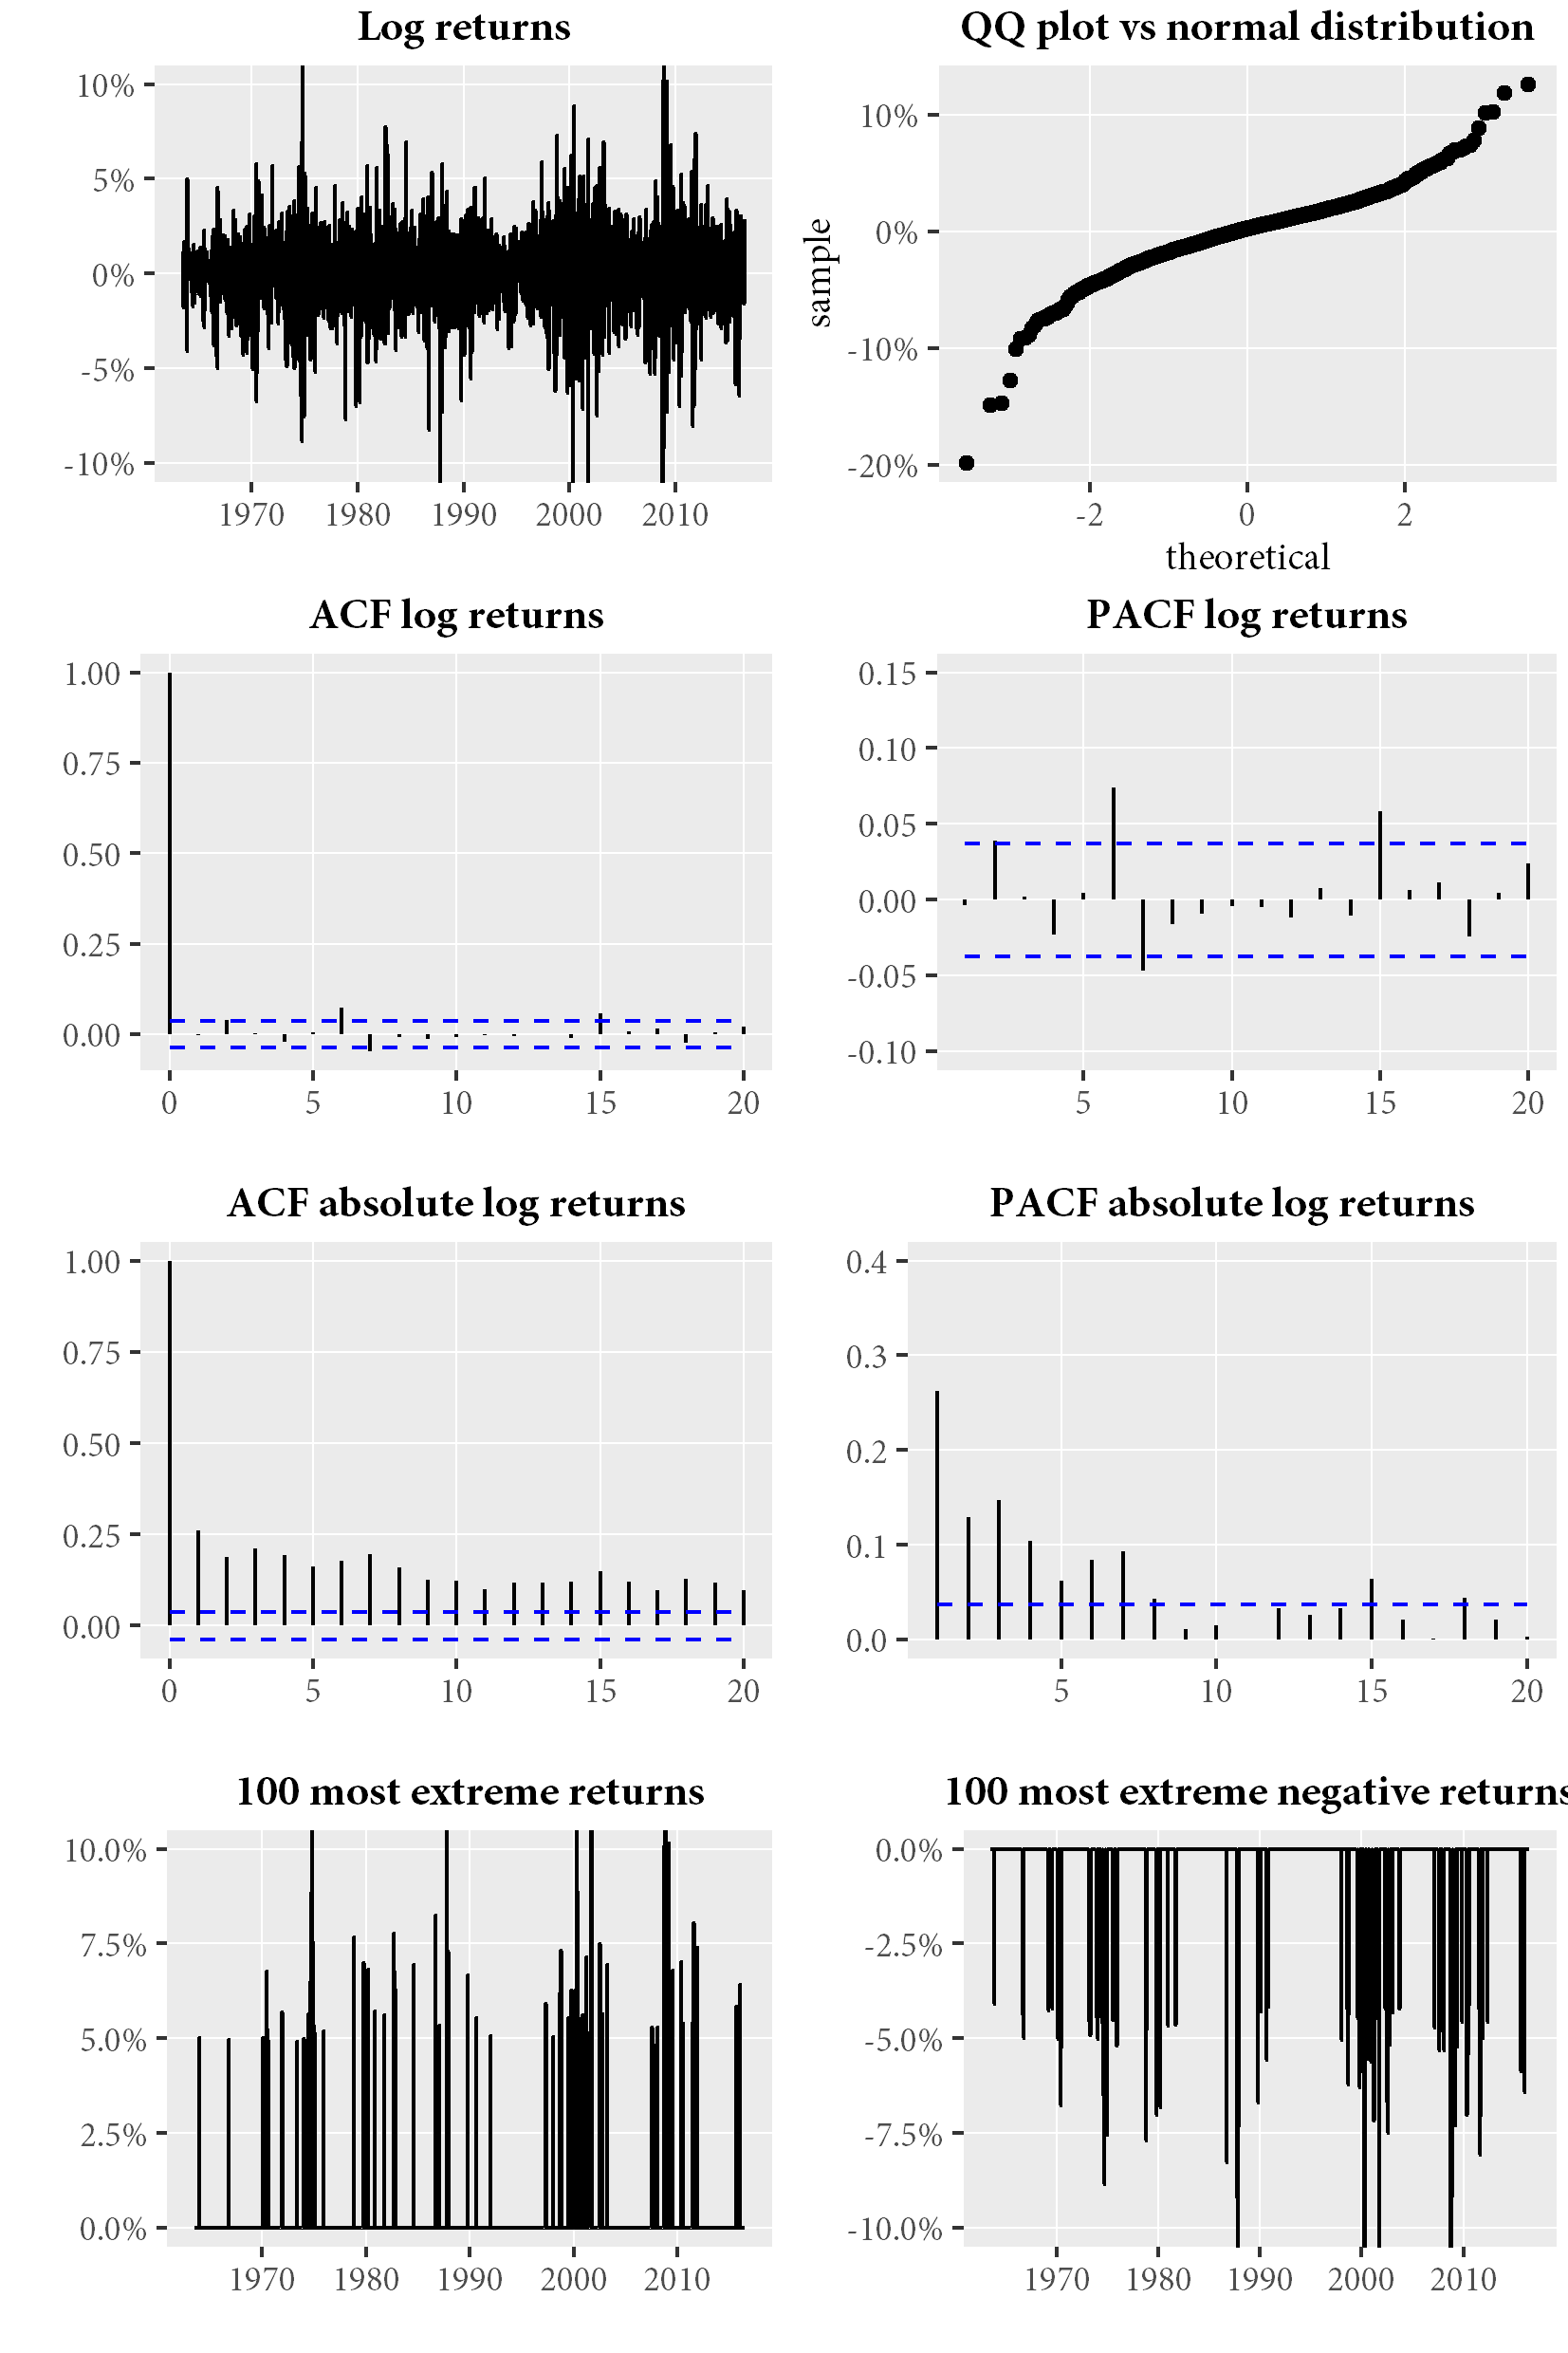
\includegraphics[scale=1]{graphics/marginal/MarginalStats.Mkt.RF.Estim.png}  
  \bottomrule
  \vspace{3mm}
  \footnotesize
  We report diagnostics plots for the marginal series. Autocorrelation and partial autocorrelation functions are plotted with 95\% confidence bounds. 
  \end{minipage}
\end{figure}
\begin{figure}[H]
  \caption{Marginal diagnostics plots - HML}
  \label{diag:marginaldiagHML}
  \toprule
  \centering
  \begin{minipage}{\textwidth}
  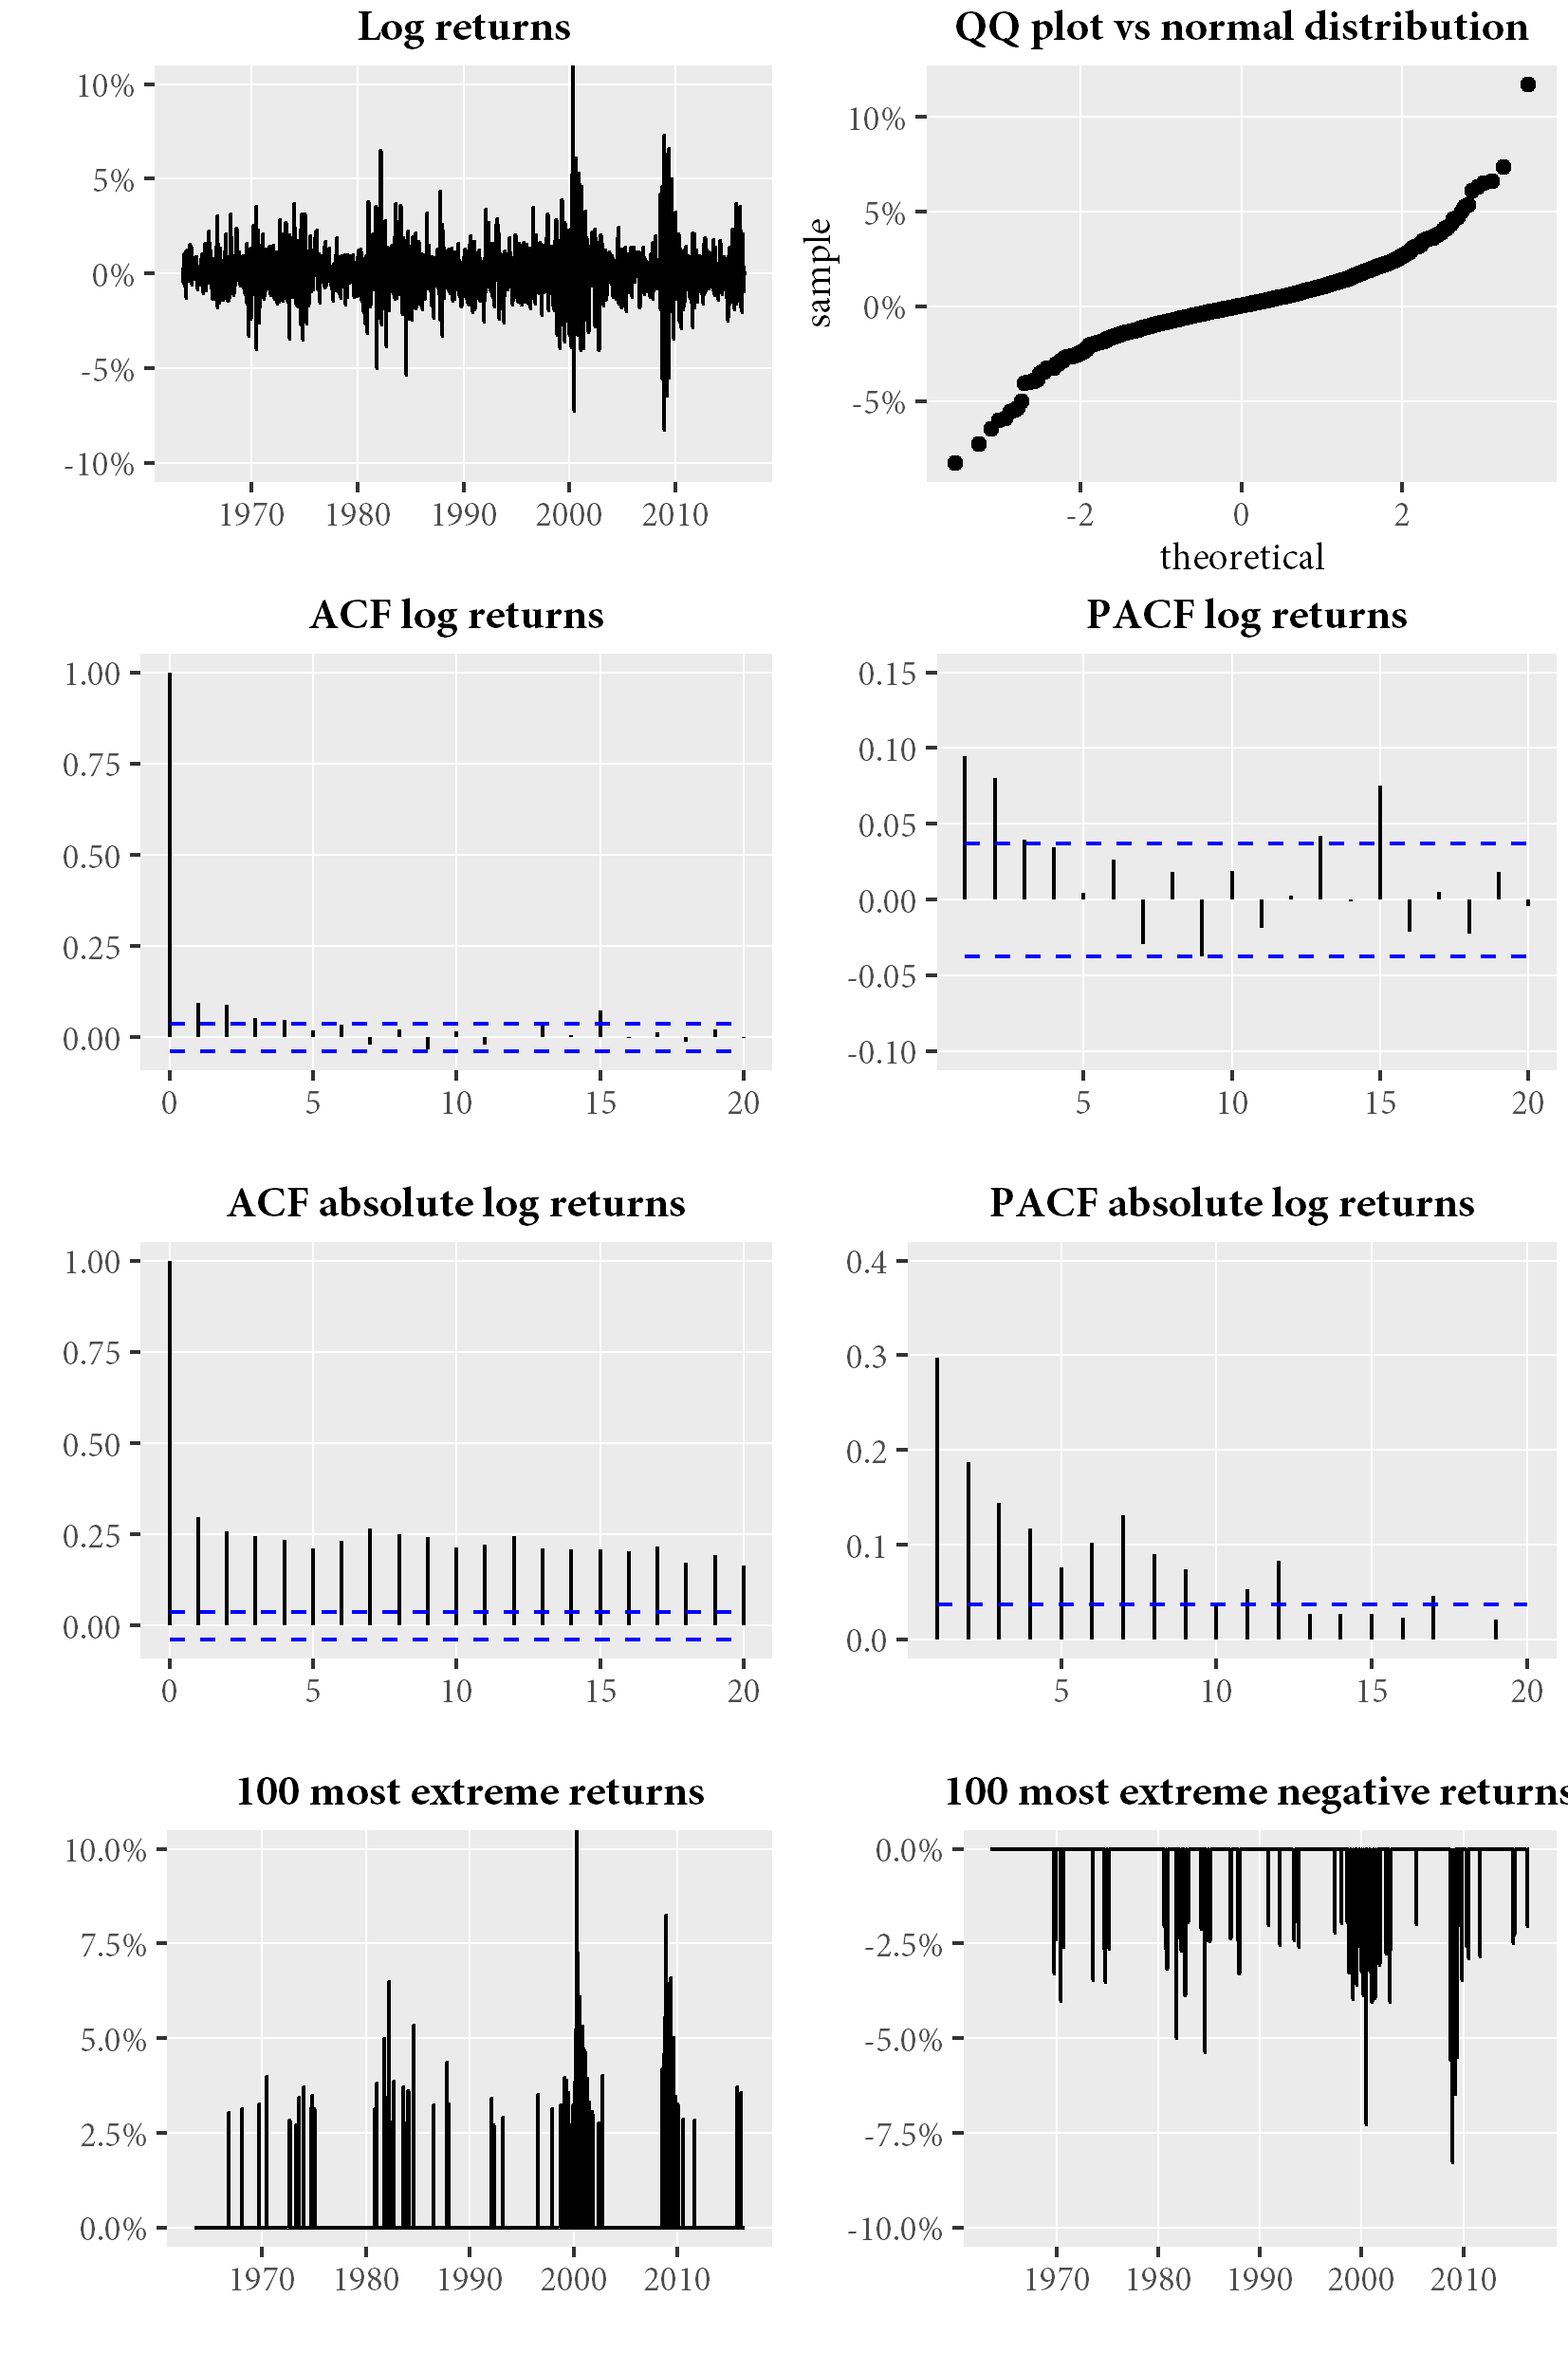
\includegraphics[scale=1]{graphics/marginal/MarginalStats.HML.Estim.png}  
  \bottomrule
  \vspace{3mm}
  \footnotesize
  We report diagnostics plots for the marginal series. Autocorrelation and partial autocorrelation functions are plotted with 95\% confidence bounds. 
  \end{minipage}
\end{figure}
\begin{figure}[H]
  \caption{Marginal diagnostics plots - SMB}
  \label{diag:marginaldiagSMB}
  \toprule
  \centering
  \begin{minipage}{\textwidth}
  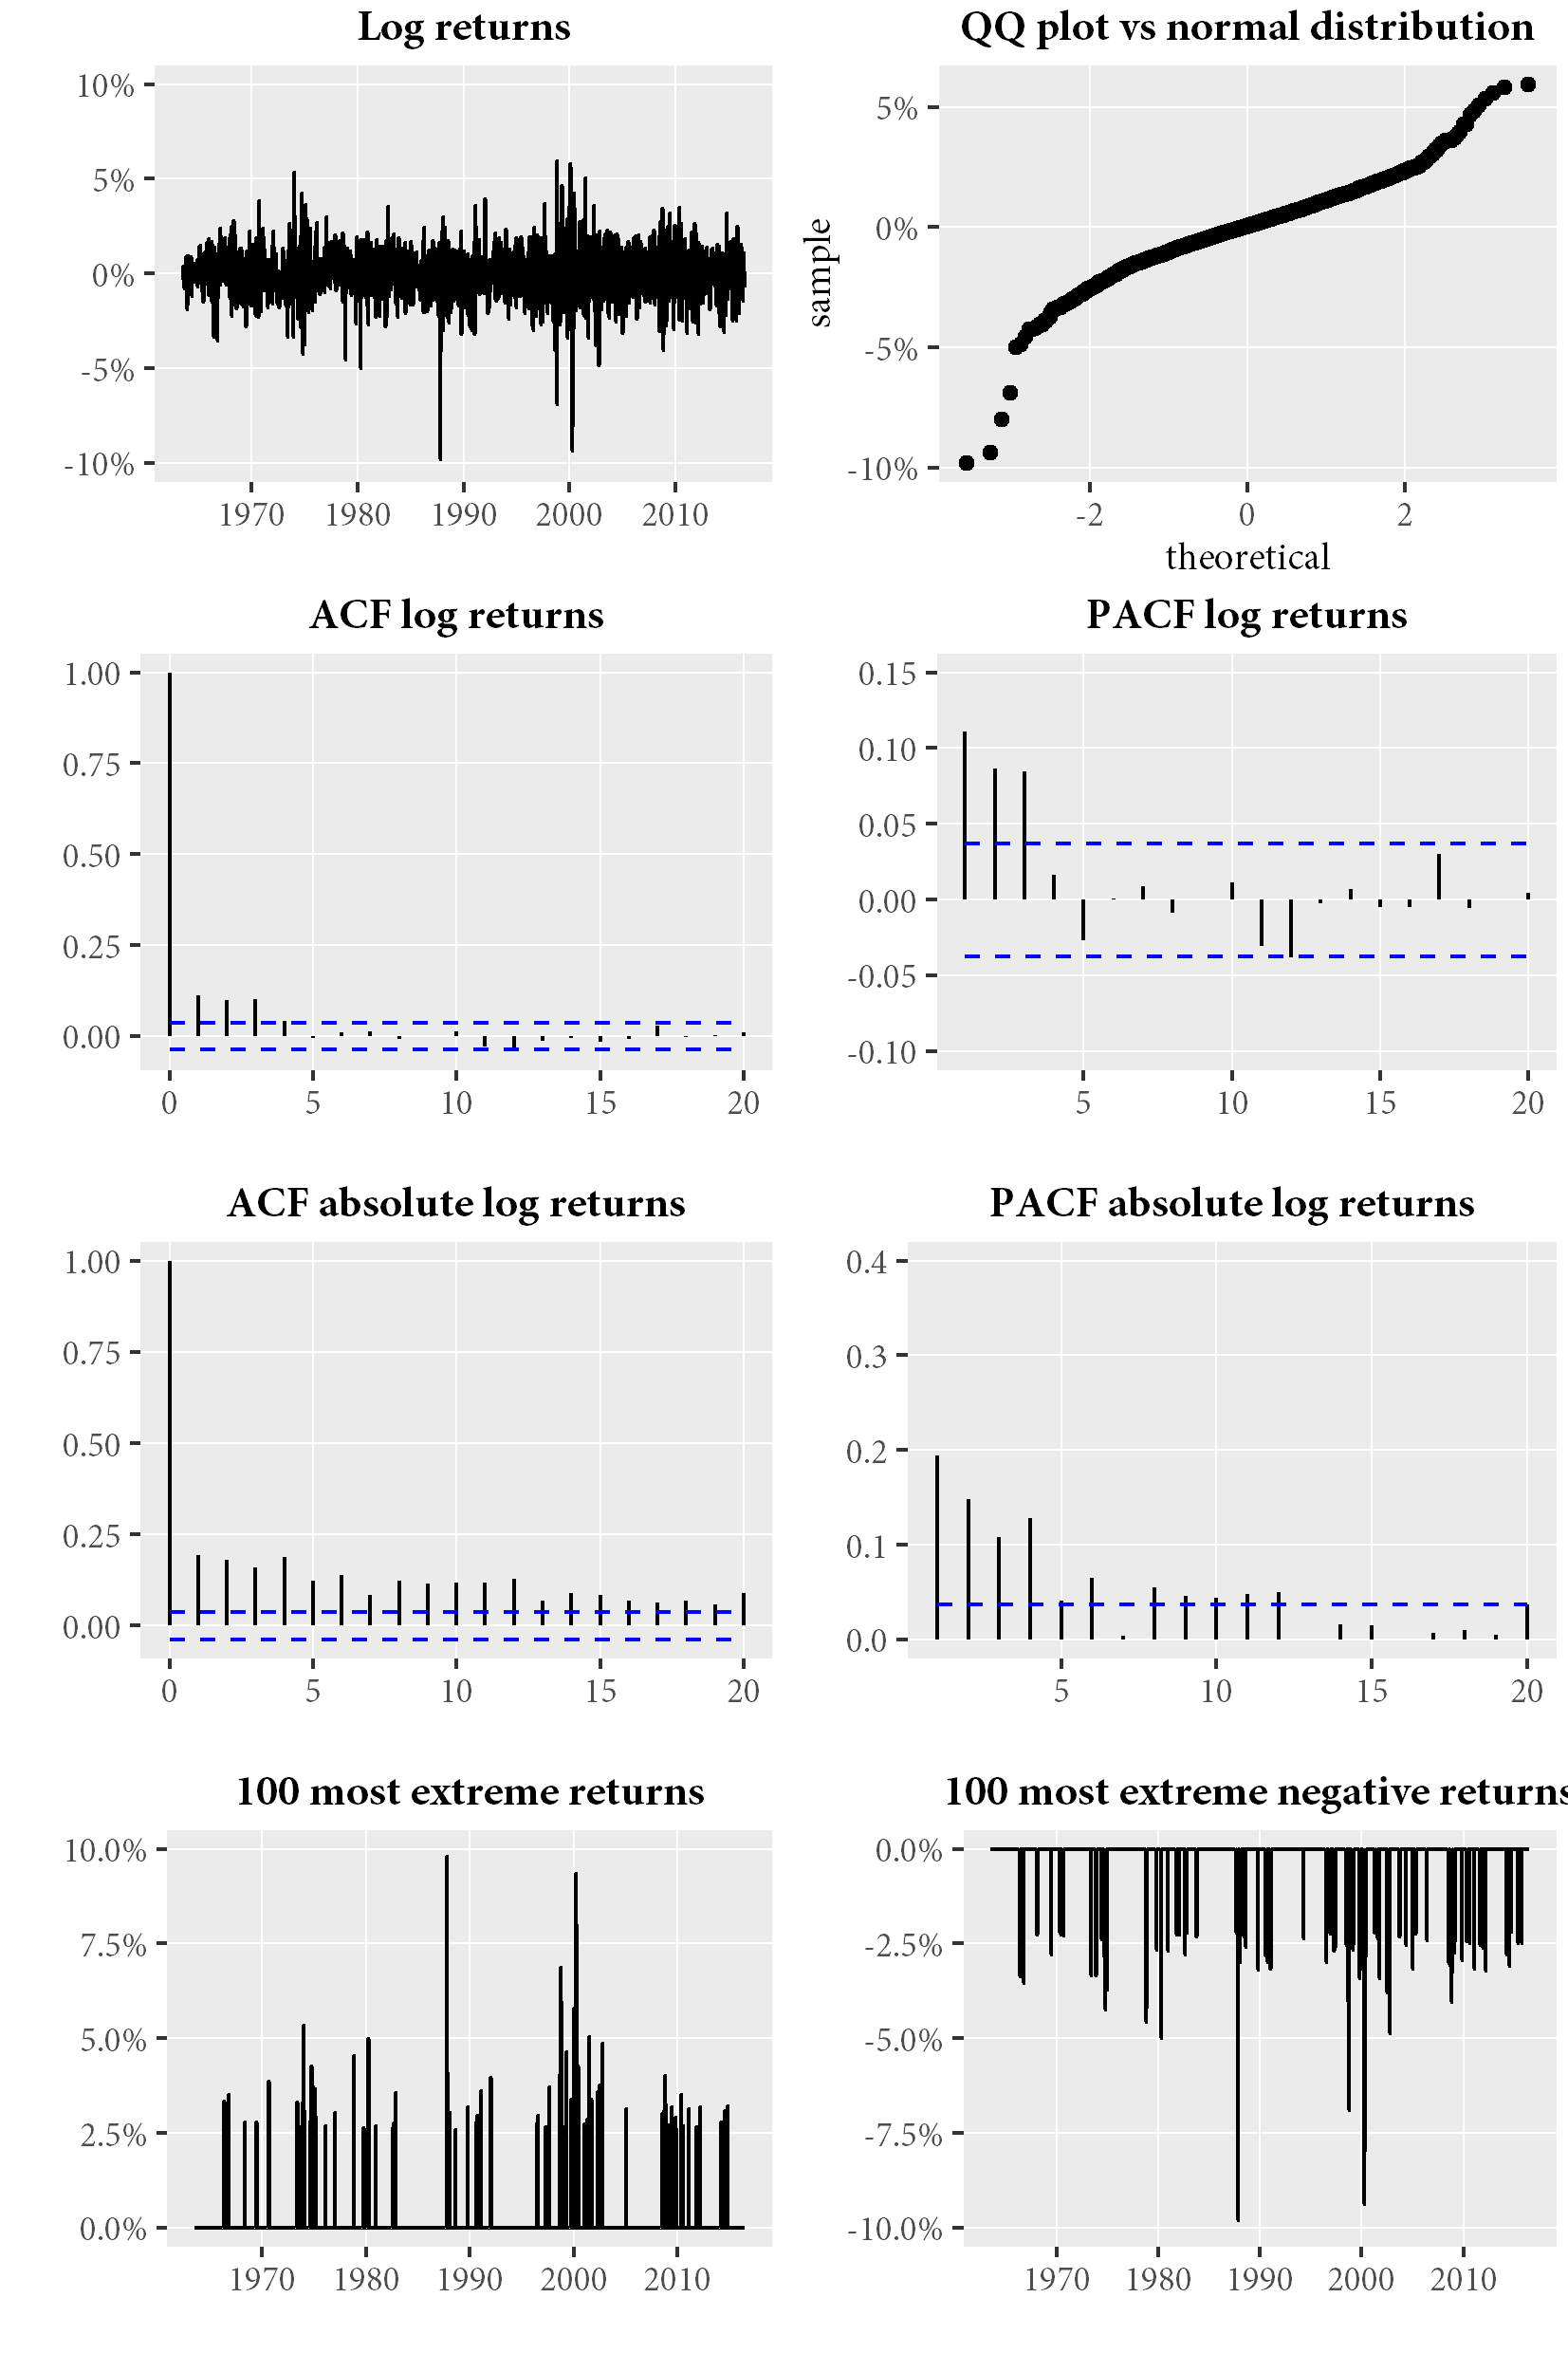
\includegraphics[scale=1]{graphics/marginal/MarginalStats.SMB.Estim.png}  
  \bottomrule
  \vspace{3mm}
  \footnotesize
  We report diagnostics plots for the marginal series. Autocorrelation and partial autocorrelation functions are plotted with 95\% confidence bounds. 
  \end{minipage}
\end{figure}
\begin{figure}[H]
  \caption{Marginal diagnostics plots - Mom}
  \label{diag:marginaldiagMom}
  \toprule
  \centering
  \begin{minipage}{\textwidth}
  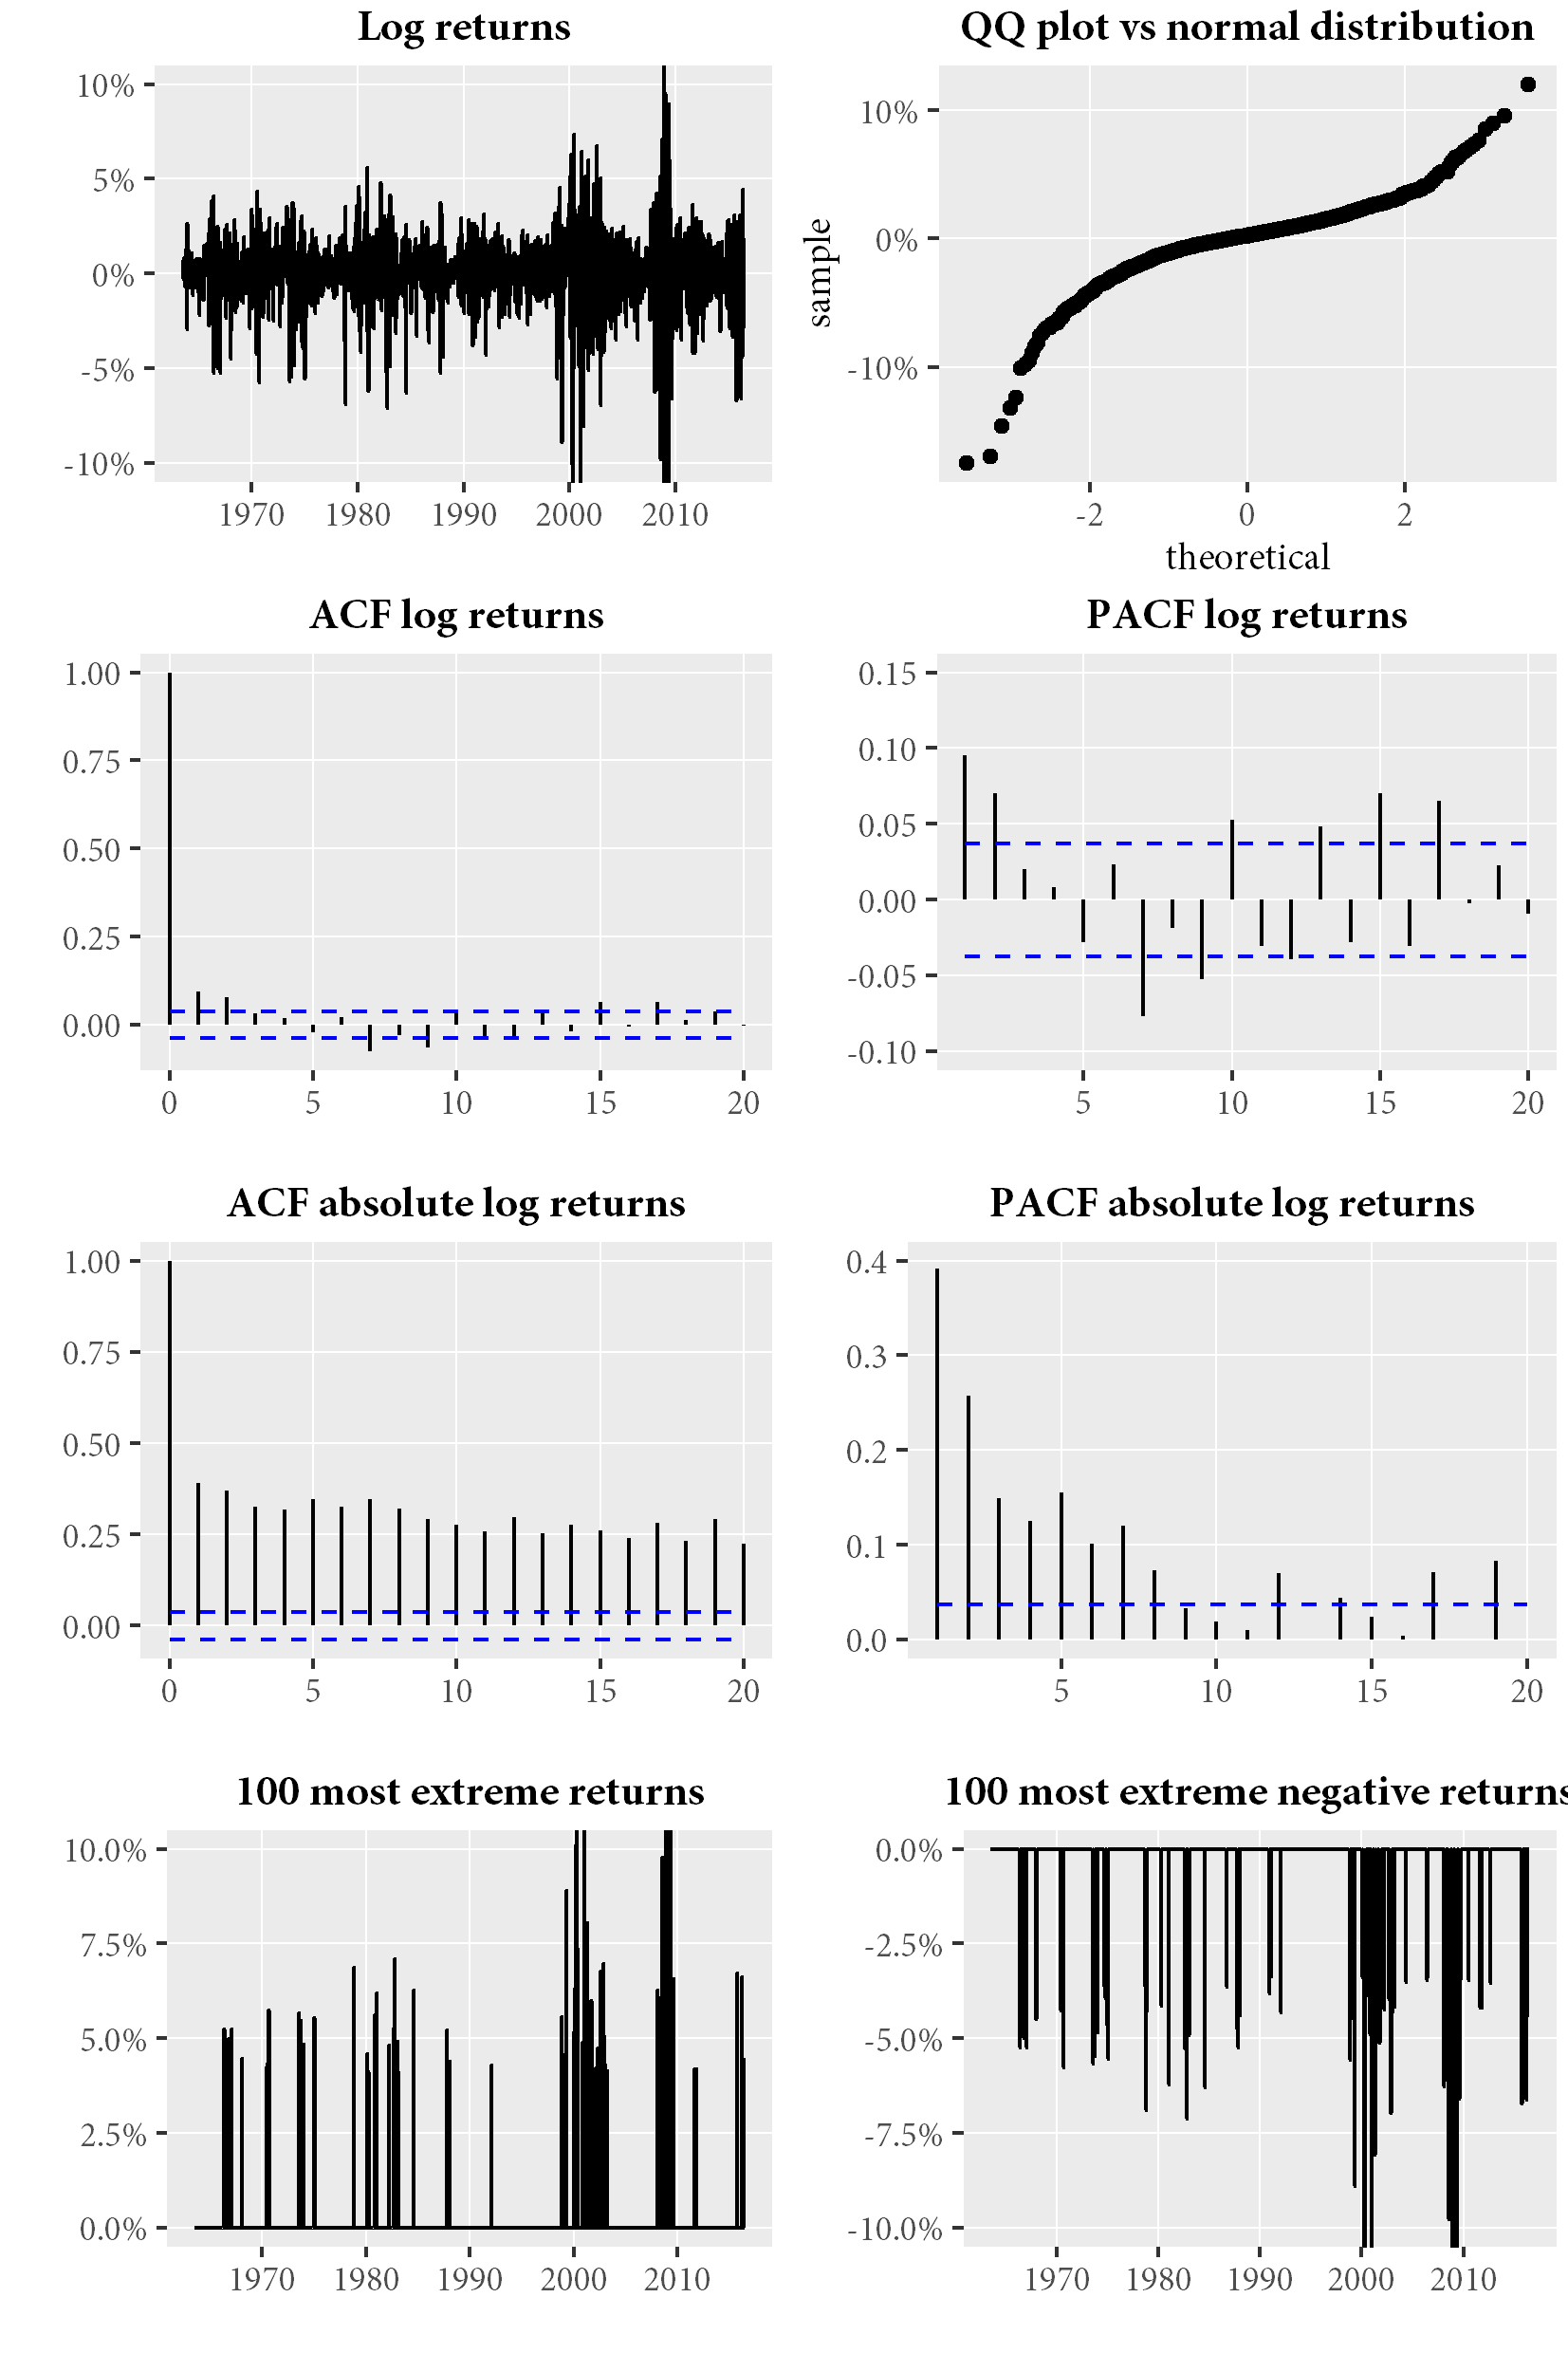
\includegraphics[scale=1]{graphics/marginal/MarginalStats.Mom.Estim.png}  
  \bottomrule
  \vspace{3mm}
  \footnotesize
  We report diagnostics plots for the marginal series. Autocorrelation and partial autocorrelation functions are plotted with 95\% confidence bounds. 
  \end{minipage}
\end{figure}
\begin{figure}[H]
  \caption{Marginal diagnostics plots - RMW}
  \label{diag:marginaldiagRMW}
  \toprule
  \centering
  \begin{minipage}{\textwidth}
  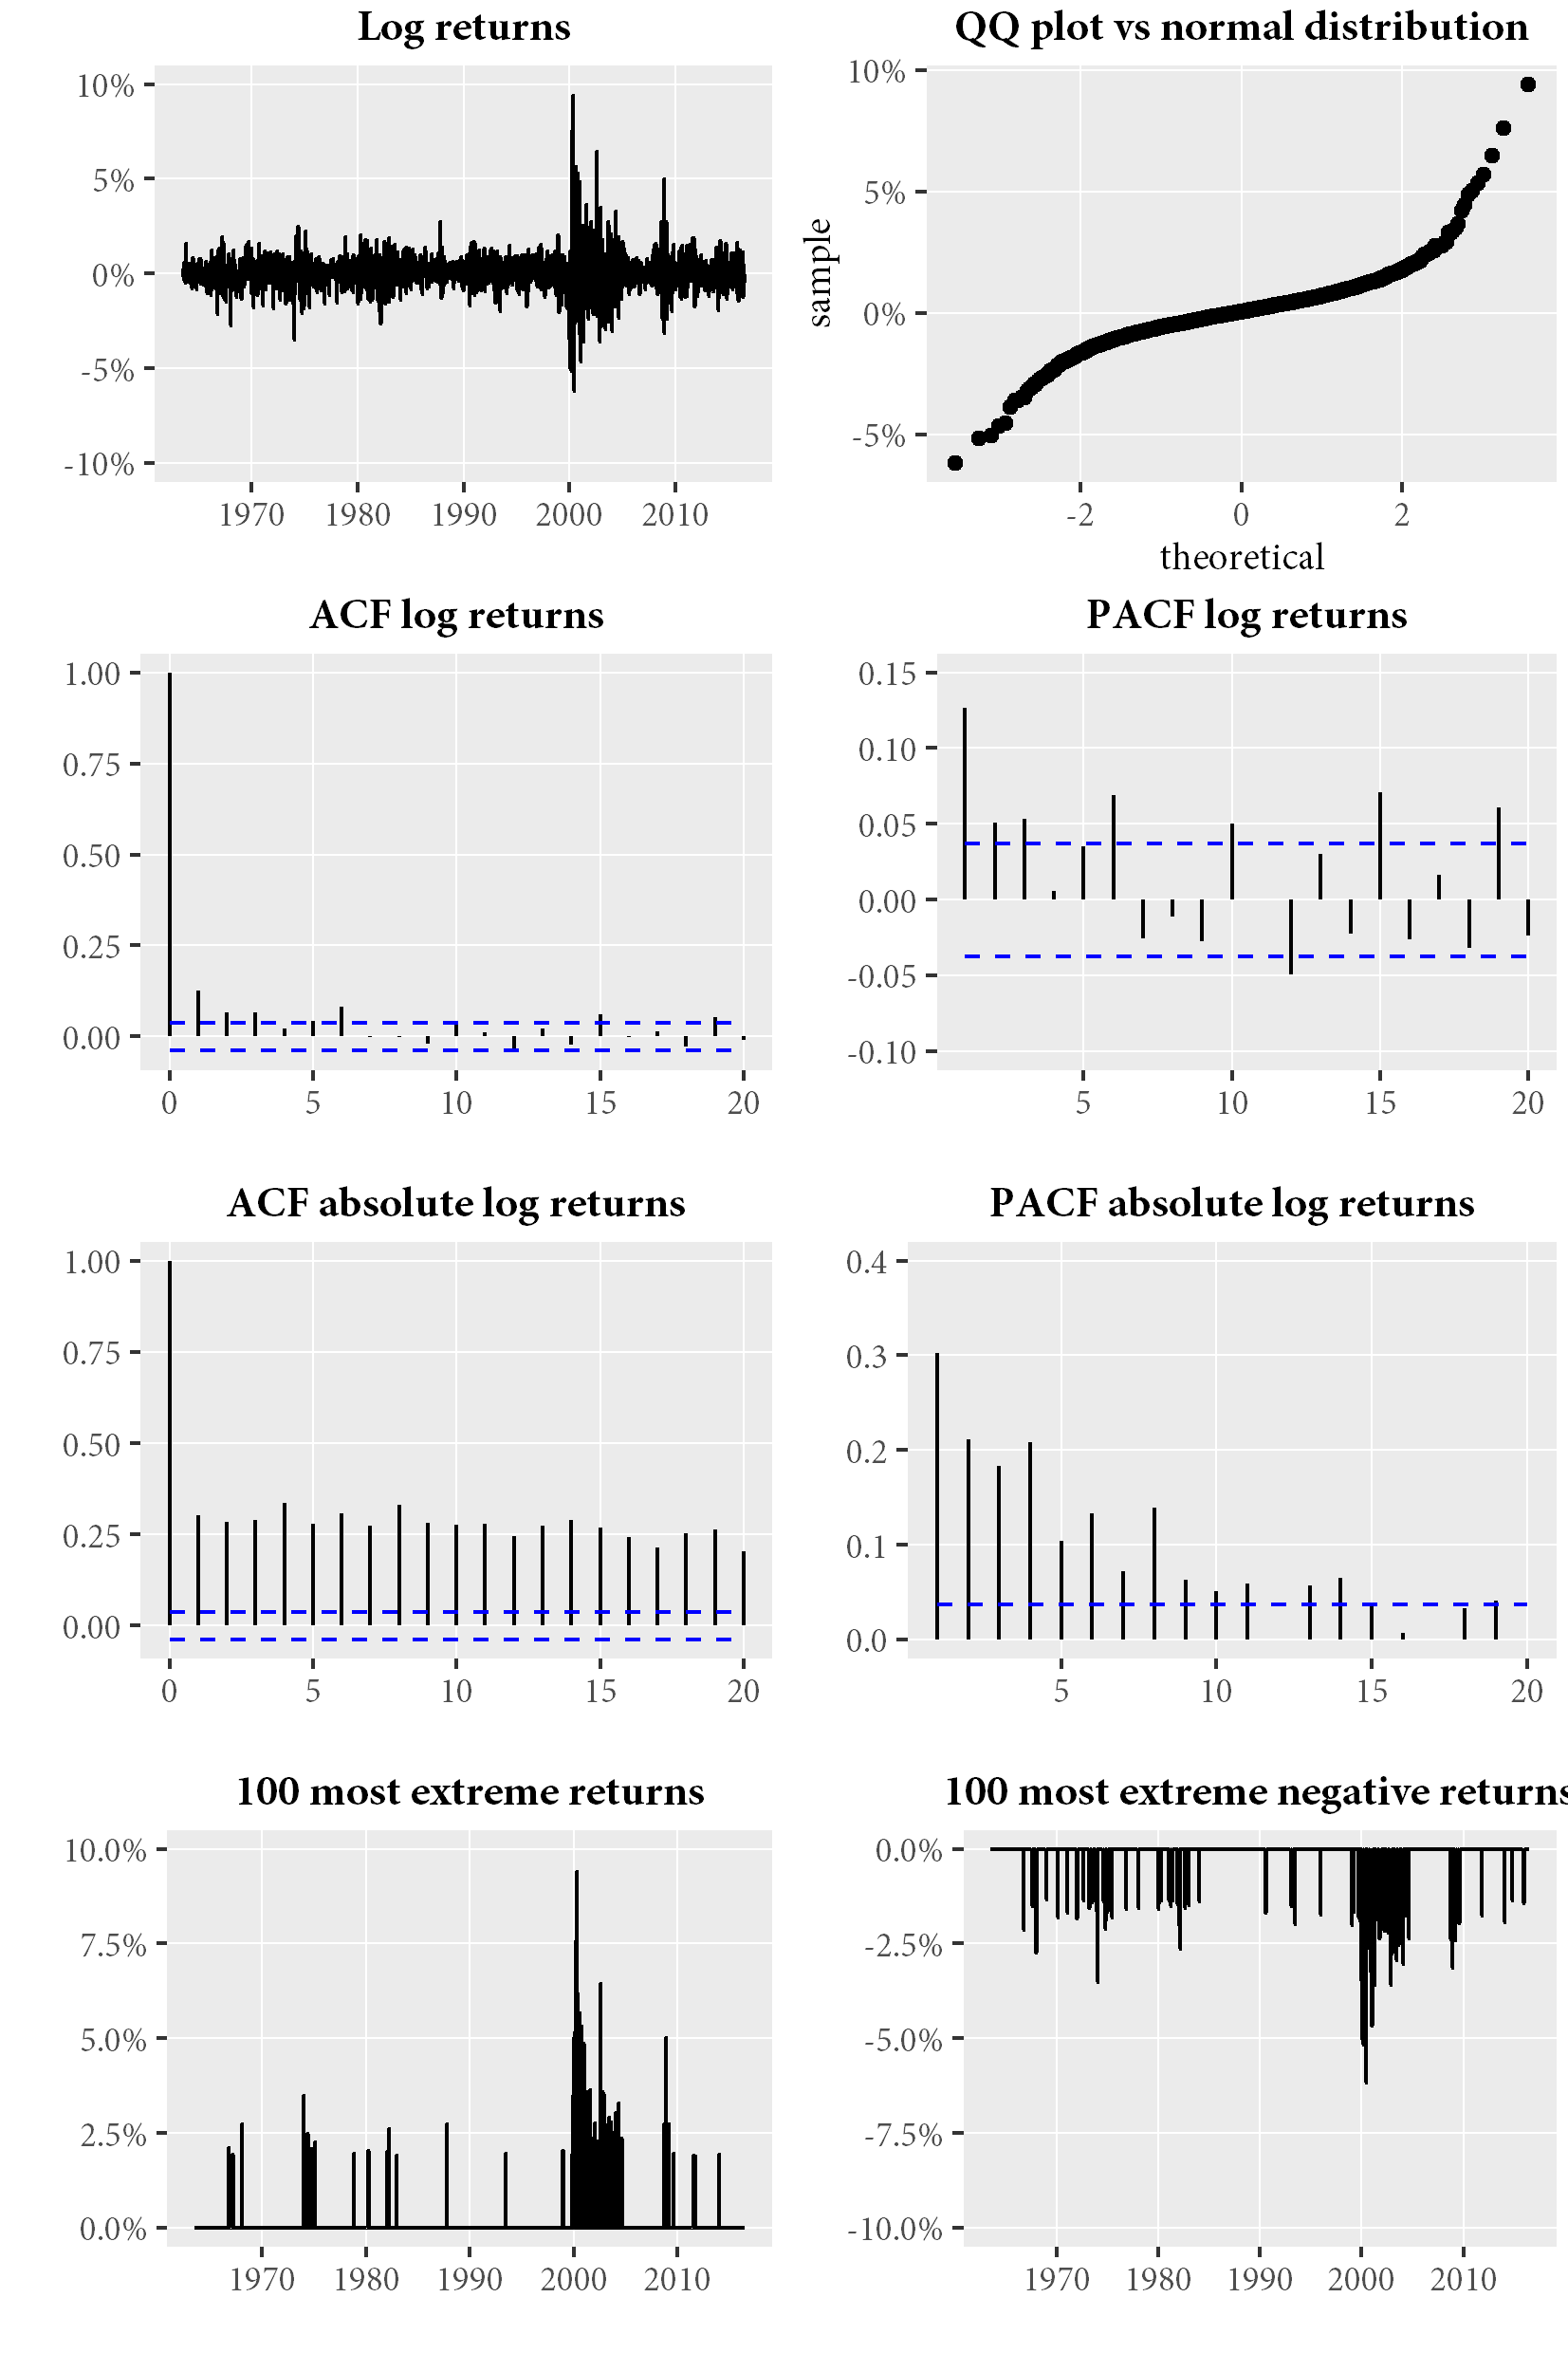
\includegraphics[scale=1]{graphics/marginal/MarginalStats.RMW.Estim.png}  
  \bottomrule
  \vspace{3mm}
  \footnotesize
  We report diagnostics plots for the marginal series. Autocorrelation and partial autocorrelation functions are plotted with 95\% confidence bounds. 
  \end{minipage}
\end{figure}
\begin{figure}[H]
  \caption{Marginal diagnostics plots - CMA}
  \label{diag:marginaldiagCMA}
  \toprule
  \centering
  \begin{minipage}{\textwidth}
  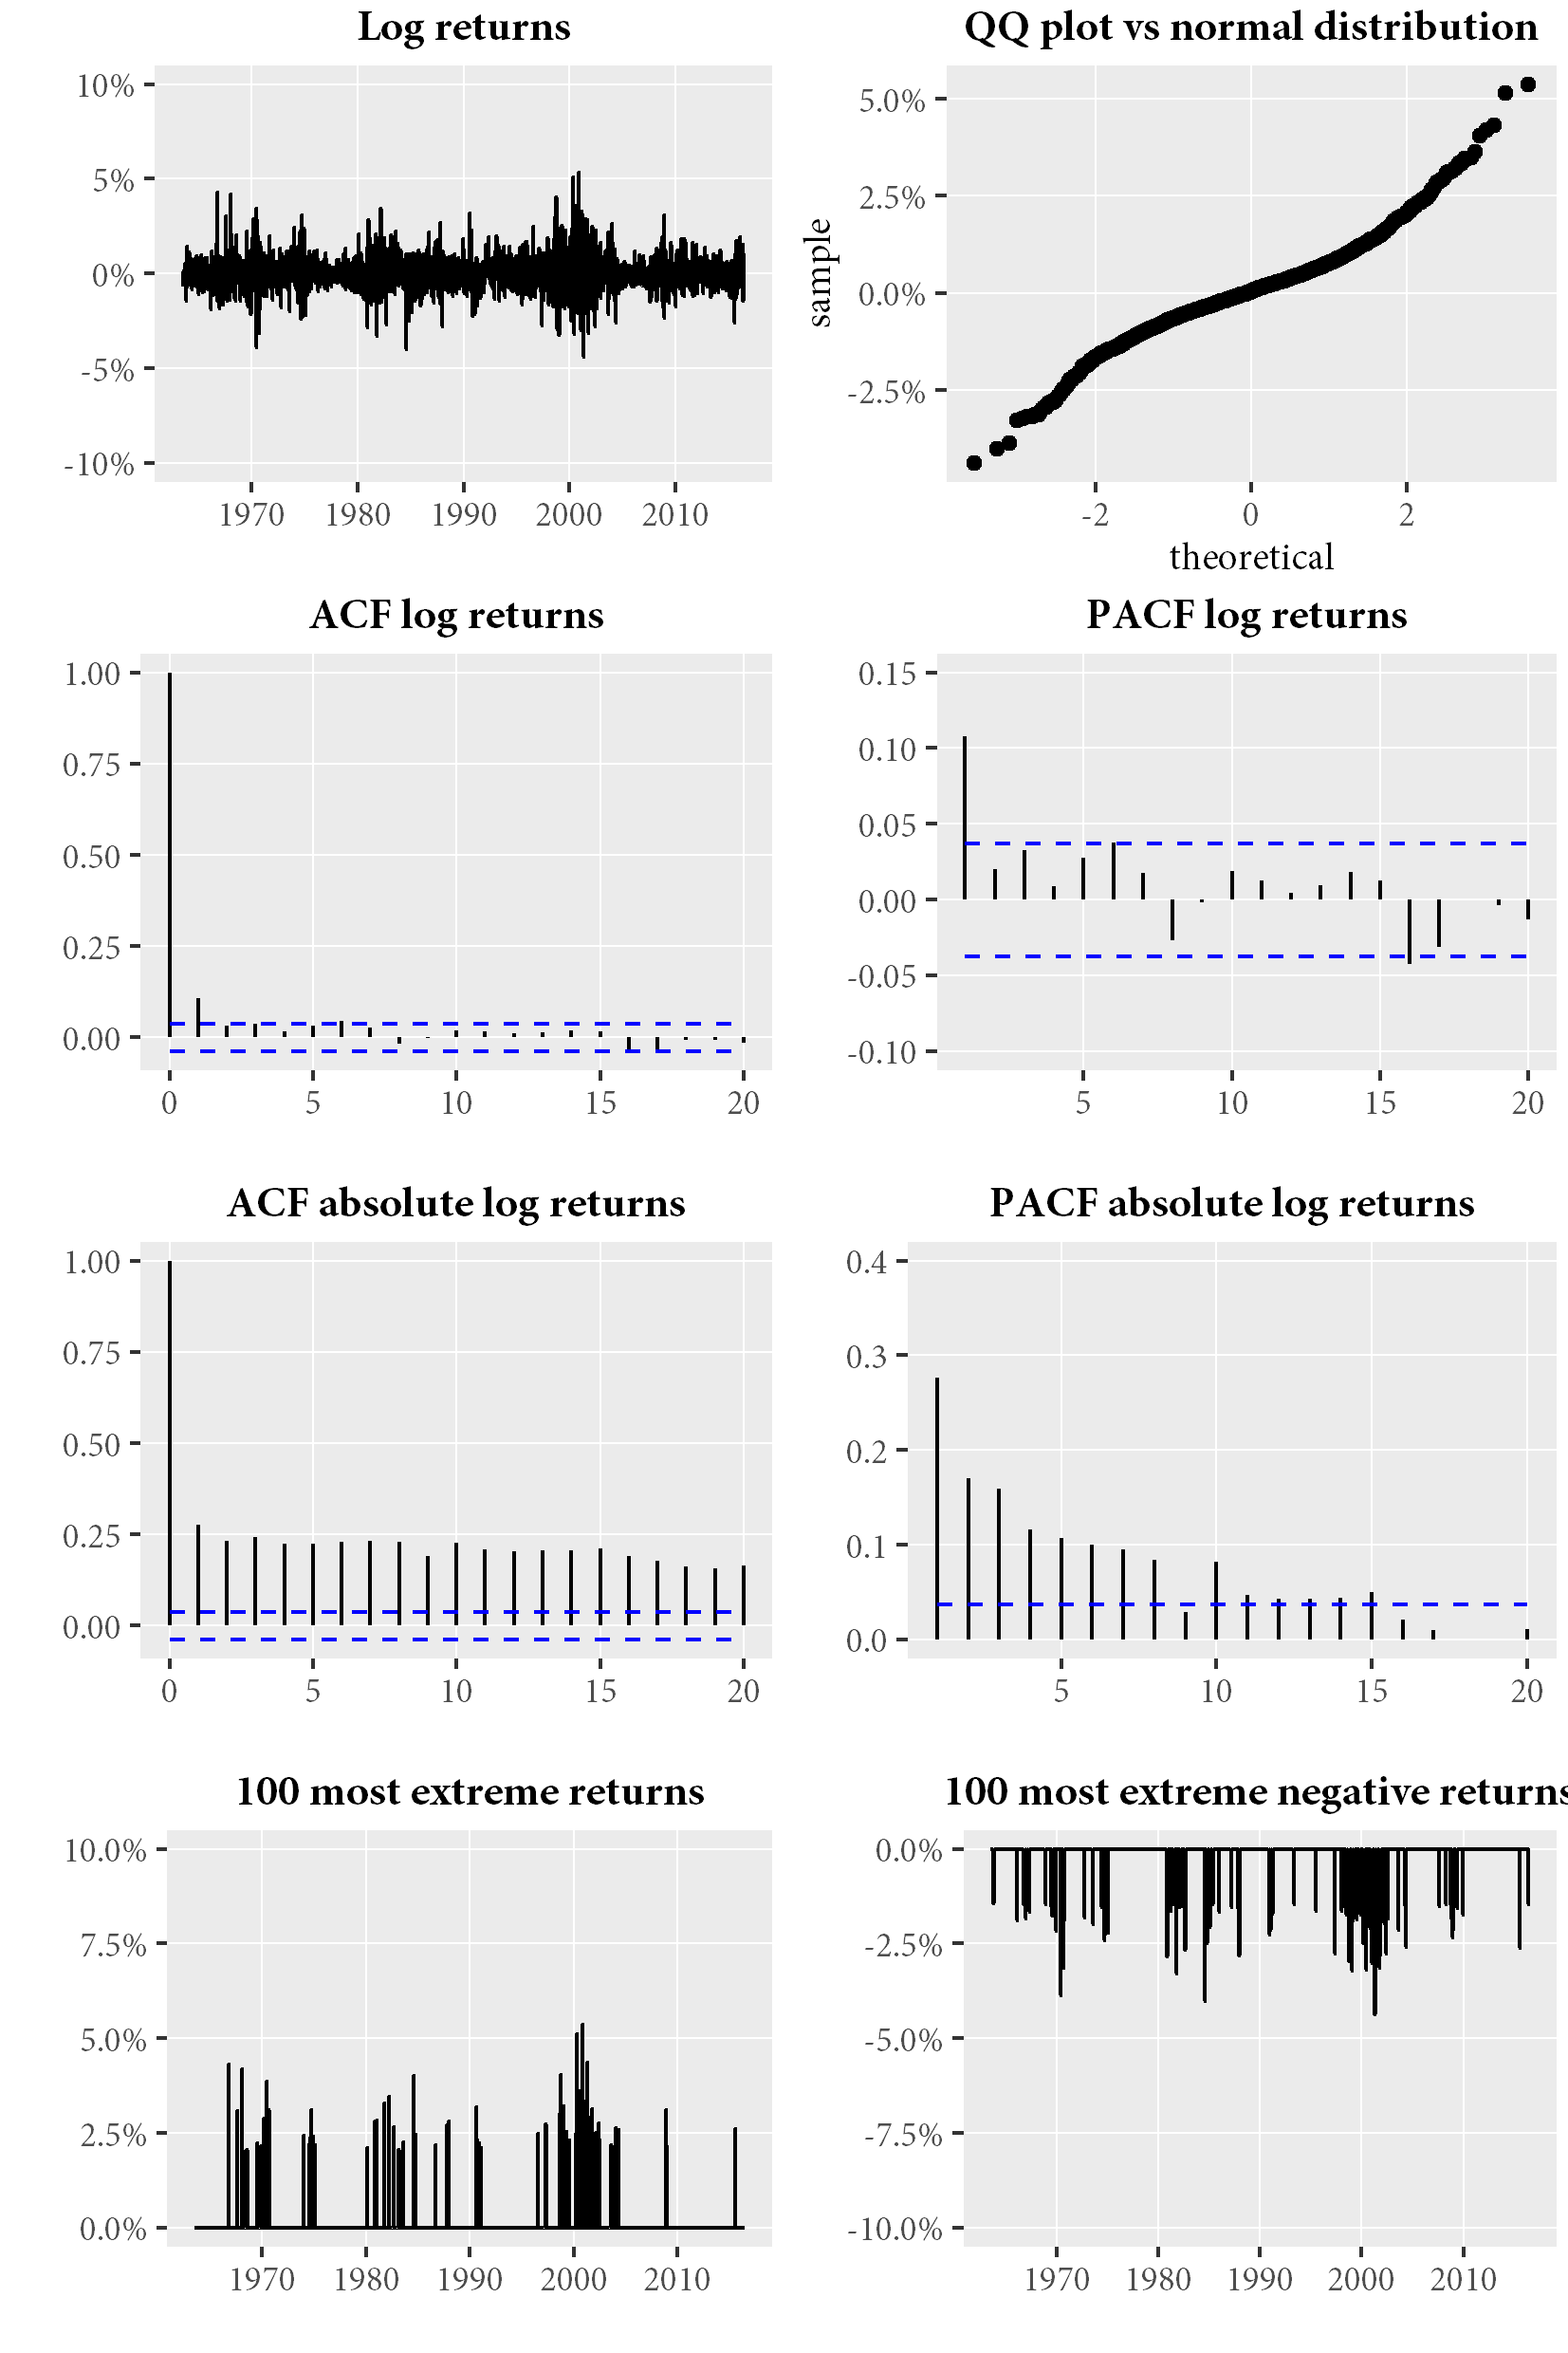
\includegraphics[scale=1]{graphics/marginal/MarginalStats.CMA.Estim.png}  
  \bottomrule
  \vspace{3mm}
  \footnotesize
  We report diagnostics plots for the marginal series. Autocorrelation and partial autocorrelation functions are plotted with 95\% confidence bounds. 
  \end{minipage}
\end{figure}
\section{Appendix G. GARCH model diagnostics}
\label{App:AppendixG}
\begin{figure}[H]
  \caption{GARCH diagnostics plots - Mkt.RF}
  \label{diag:garchdiagMkt.RF}
  \toprule
  \centering
  \begin{minipage}{\textwidth}
  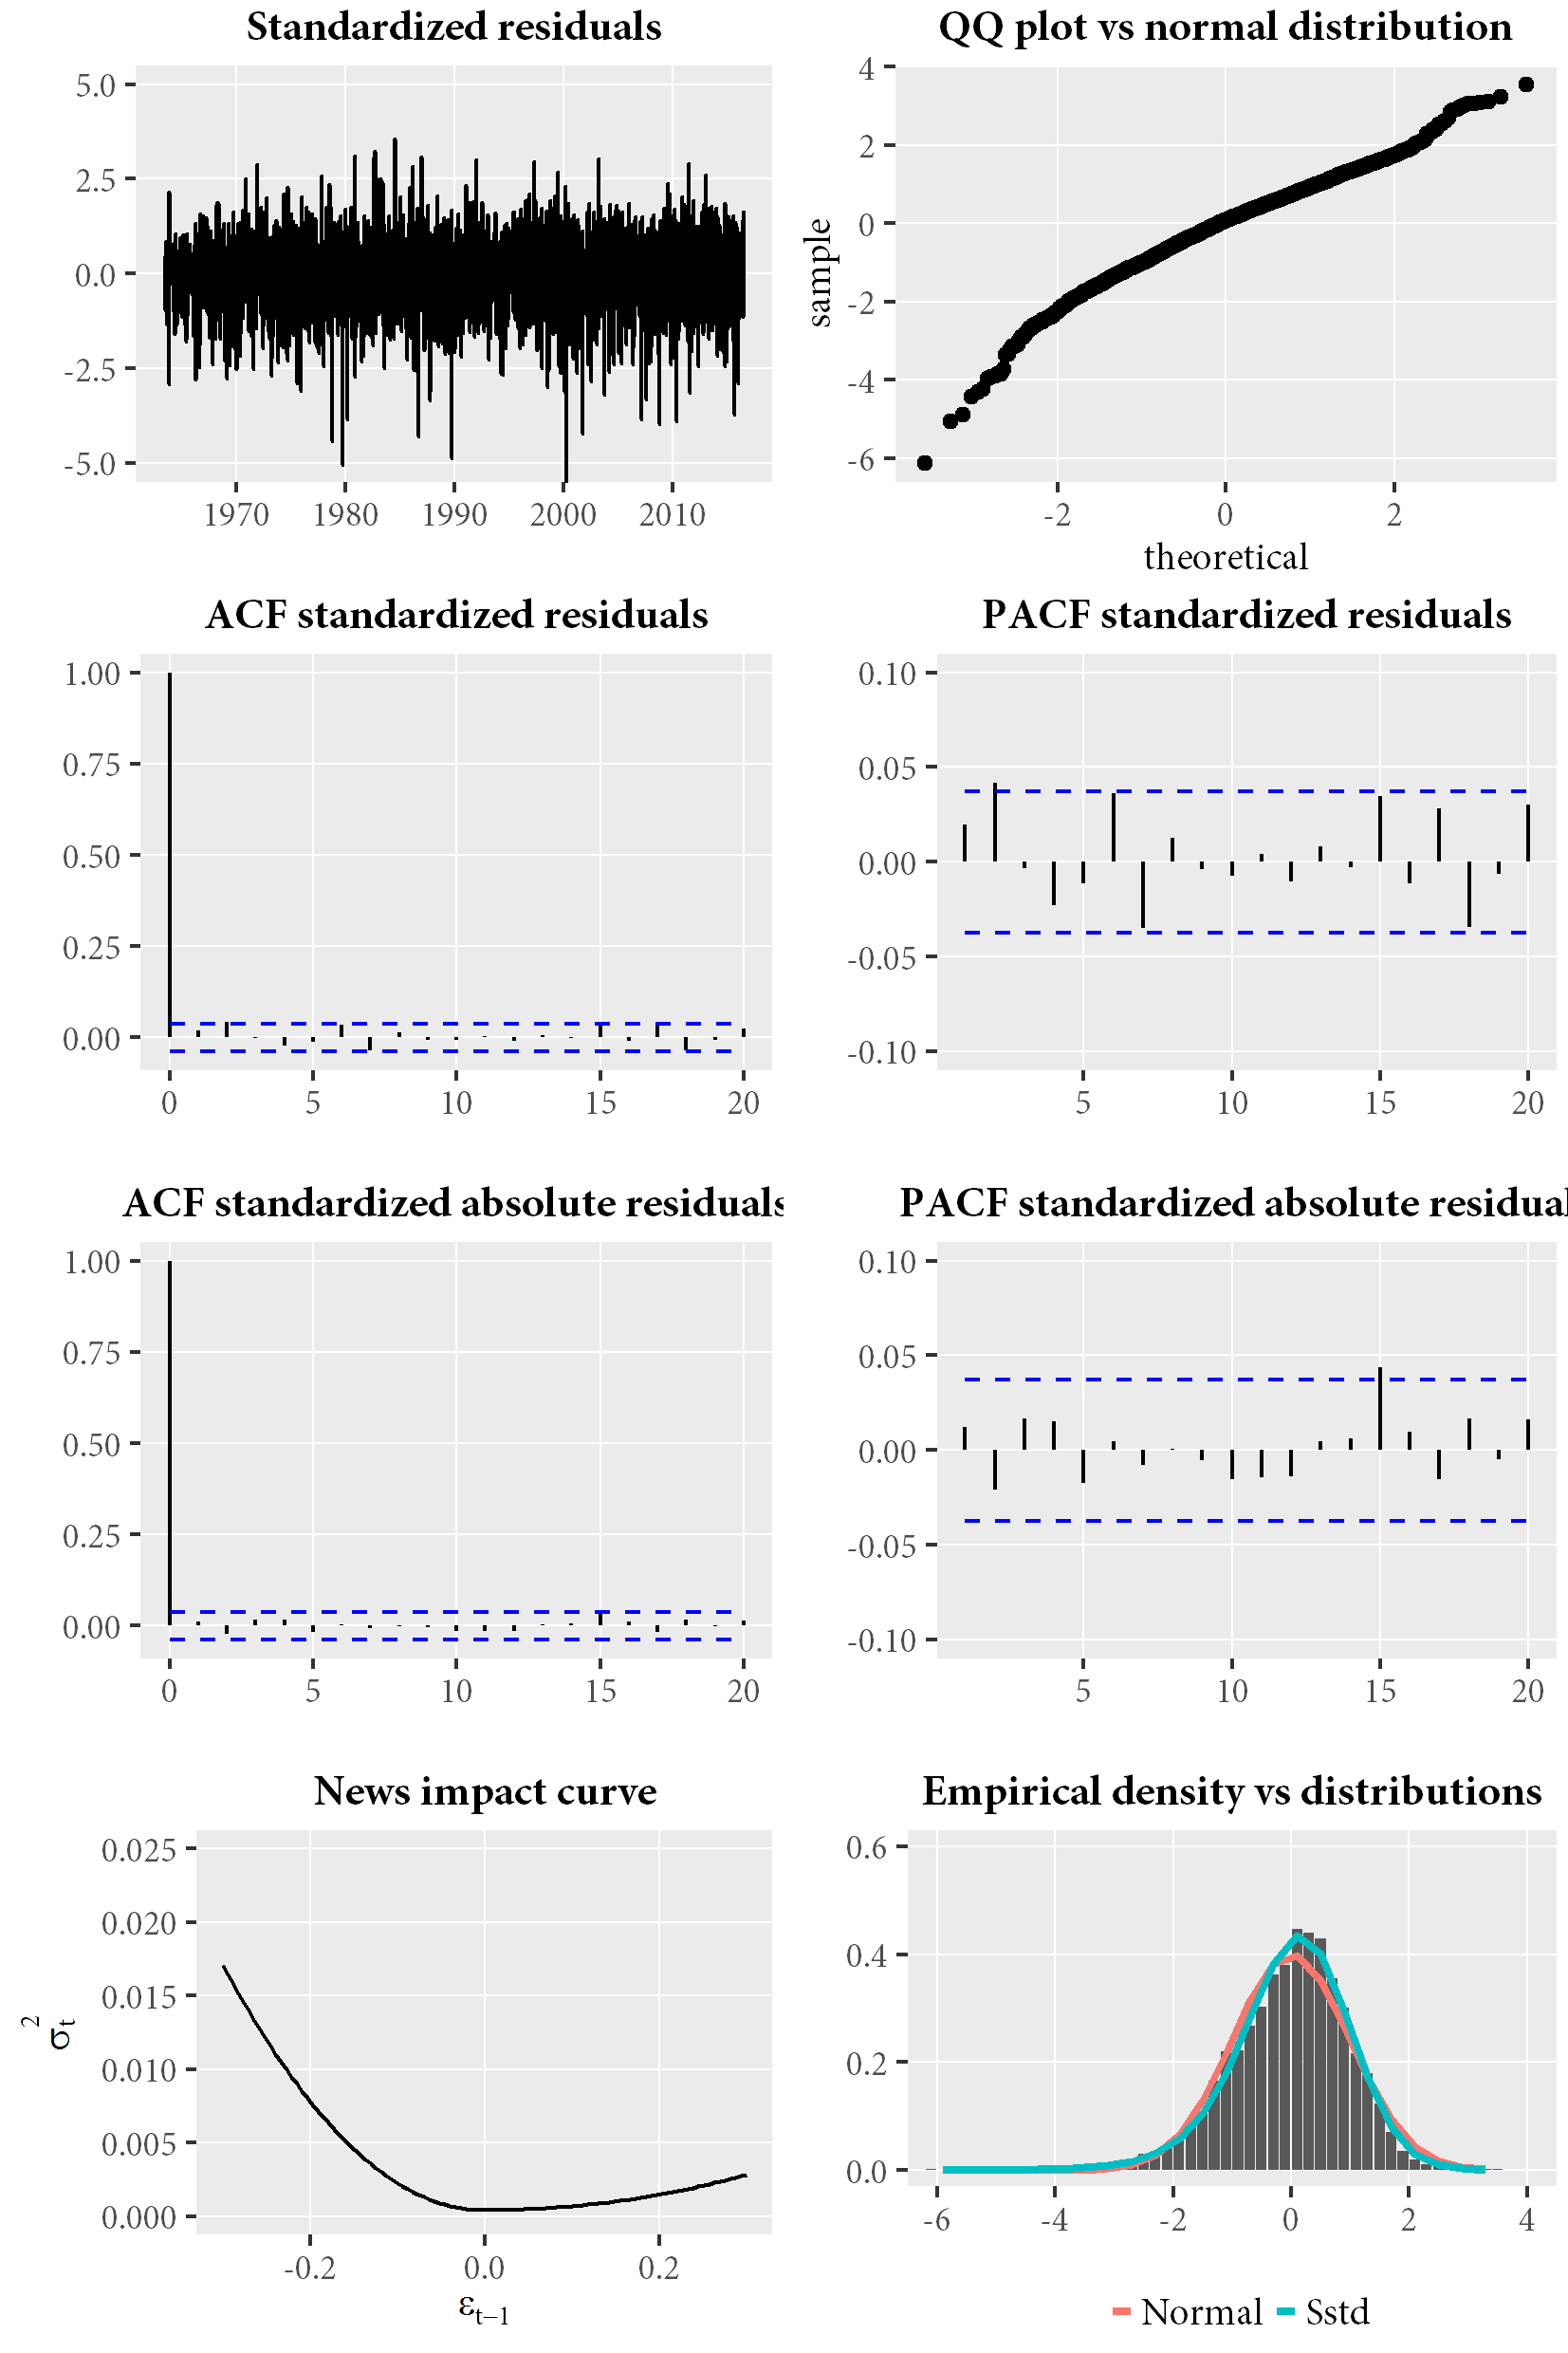
\includegraphics[scale=1]{graphics/garch/garch_diagnosticsMkt.RF.png}  
  \bottomrule
  \vspace{3mm}
  \footnotesize
  We report diagnostics plots for the ARMA-GJR-GARCH residuals. Autocorrelation and partial autocorrelation functions are plotted with 95\% confidence bounds.
  \end{minipage}
\end{figure}
\begin{figure}[H]
  \caption{GARCH diagnostics plots - HML}
  \label{diag:garchdiagHML}
  \toprule
  \centering
  \begin{minipage}{\textwidth}
  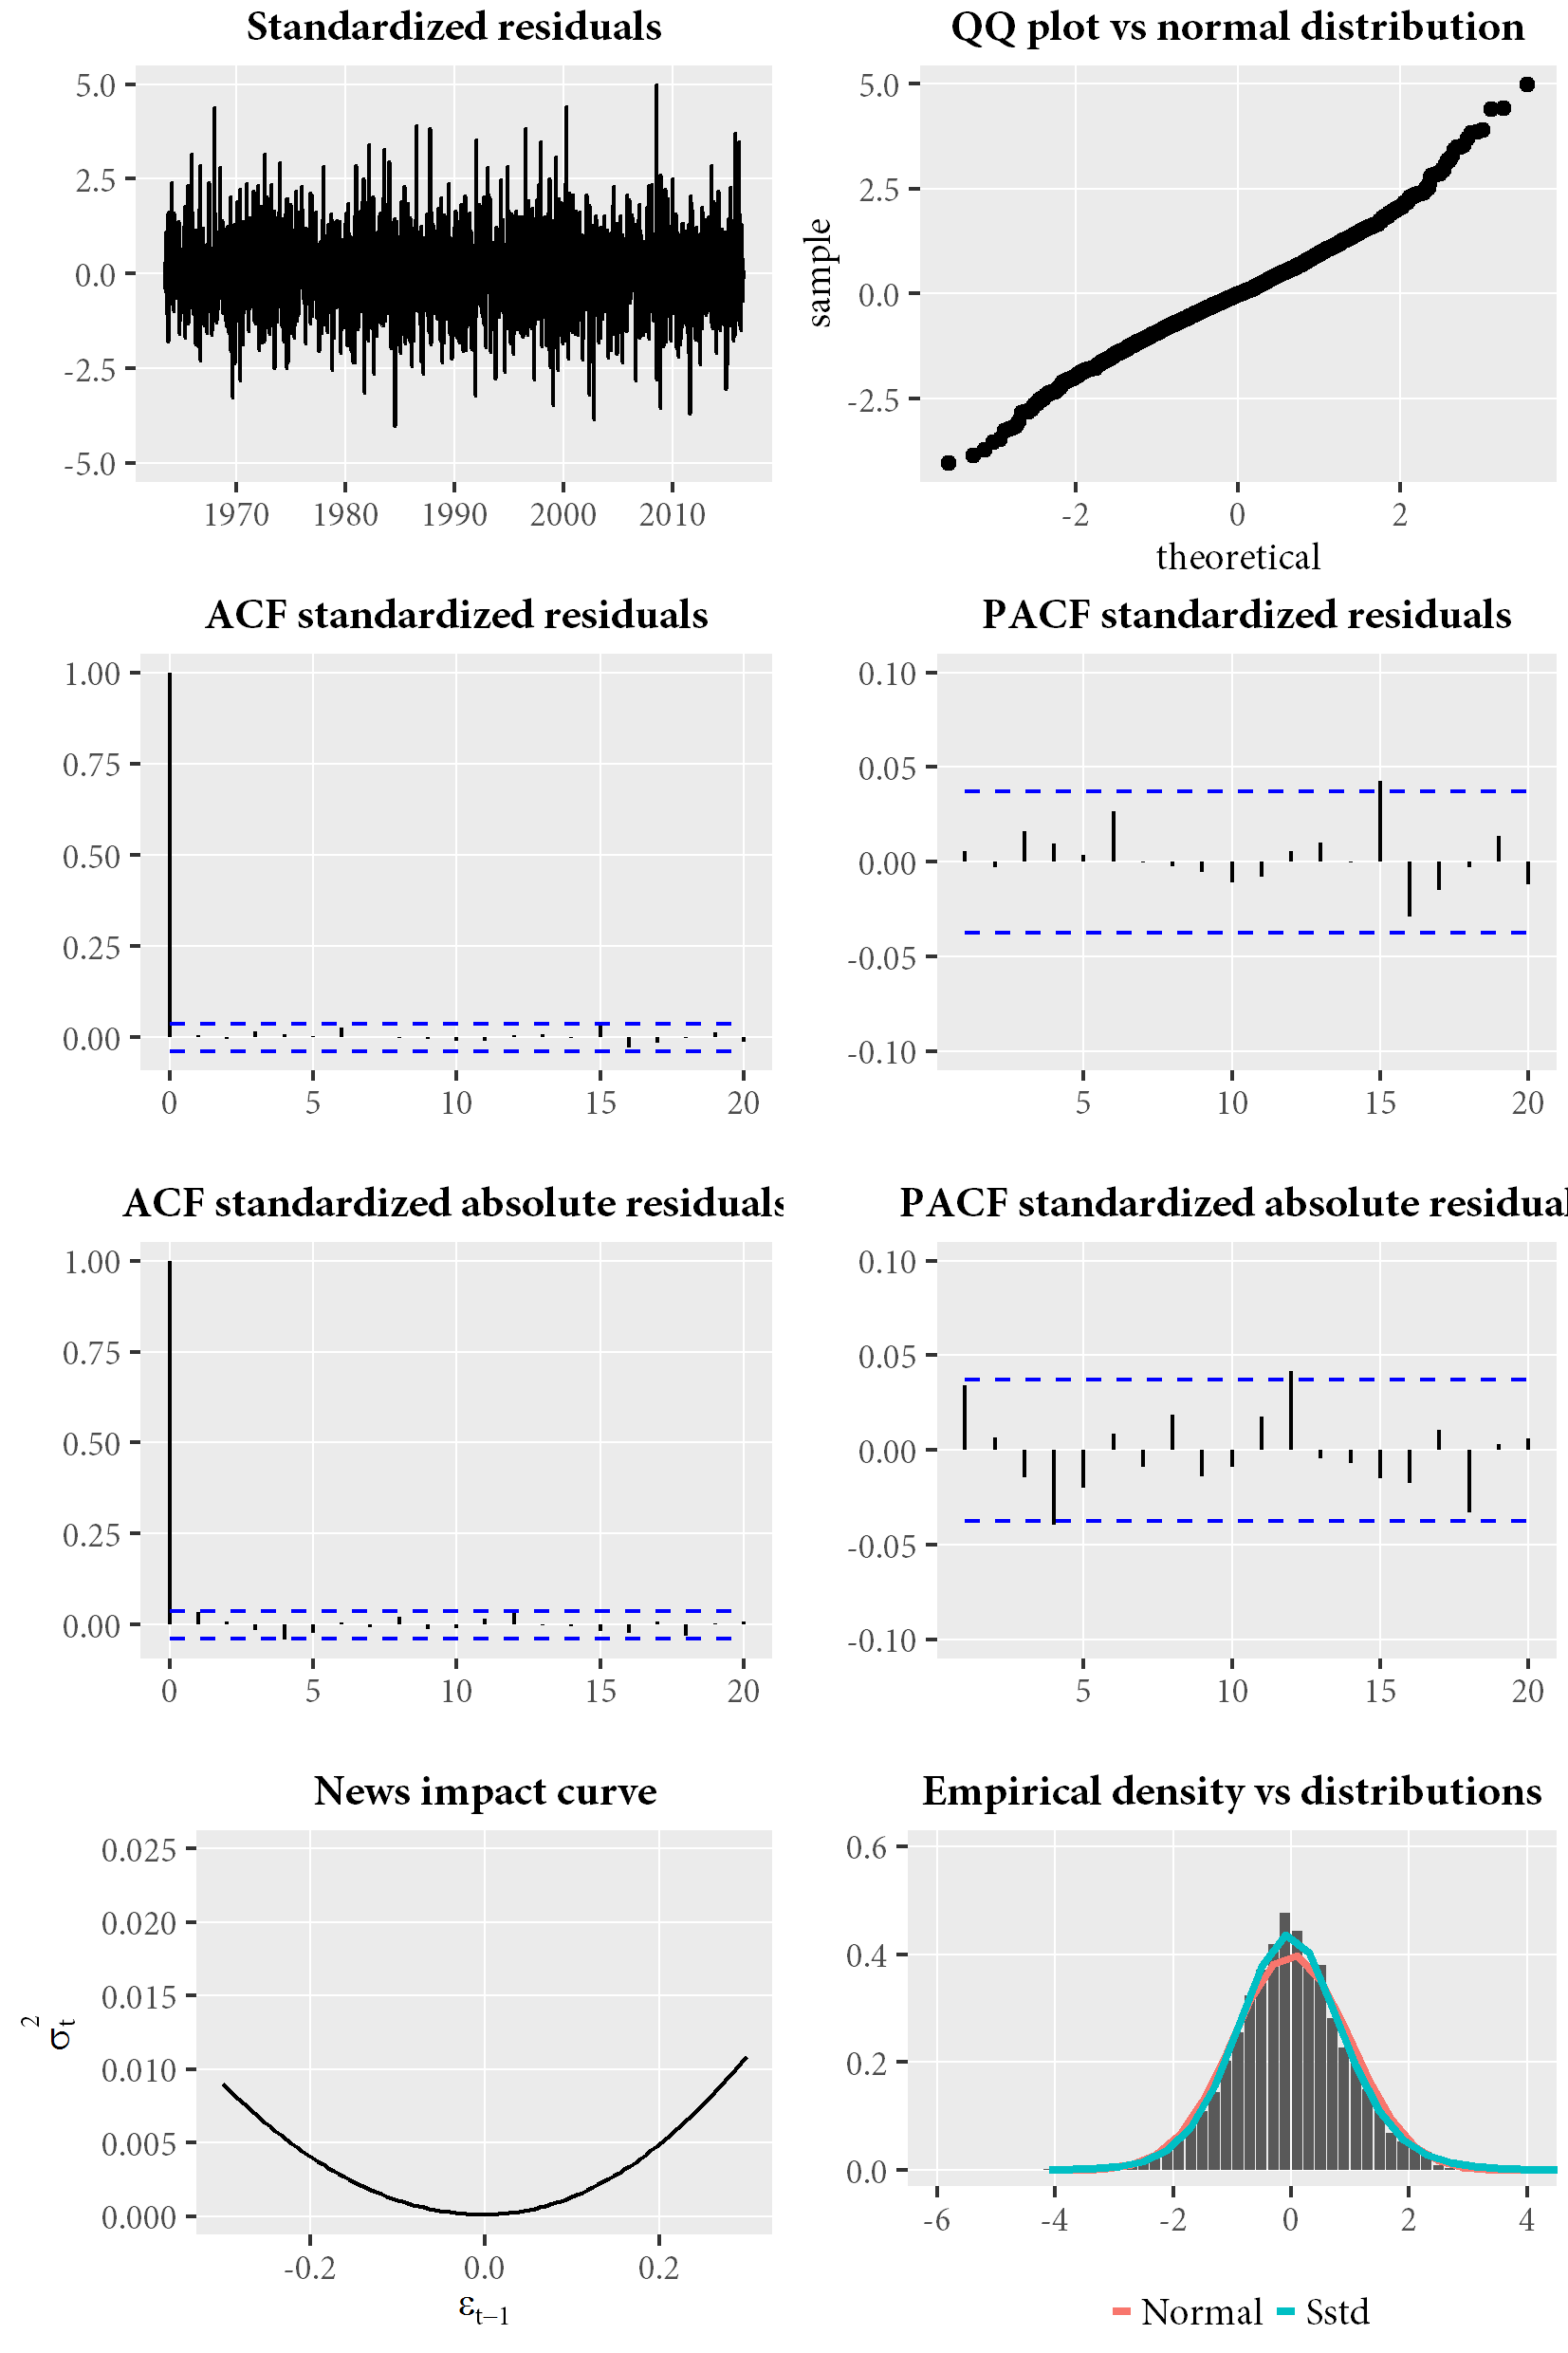
\includegraphics[scale=1]{graphics/garch/garch_diagnosticsHML.png}  
  \bottomrule
  \vspace{3mm}
  \footnotesize
  We report diagnostics plots for the ARMA-GJR-GARCH residuals. Autocorrelation and partial autocorrelation functions are plotted with 95\% confidence bounds.
  \end{minipage}
\end{figure}
\begin{figure}[H]
  \caption{GARCH diagnostics plots - SMB}
  \label{diag:garchdiagSMB}
  \toprule
  \centering
  \begin{minipage}{\textwidth}
  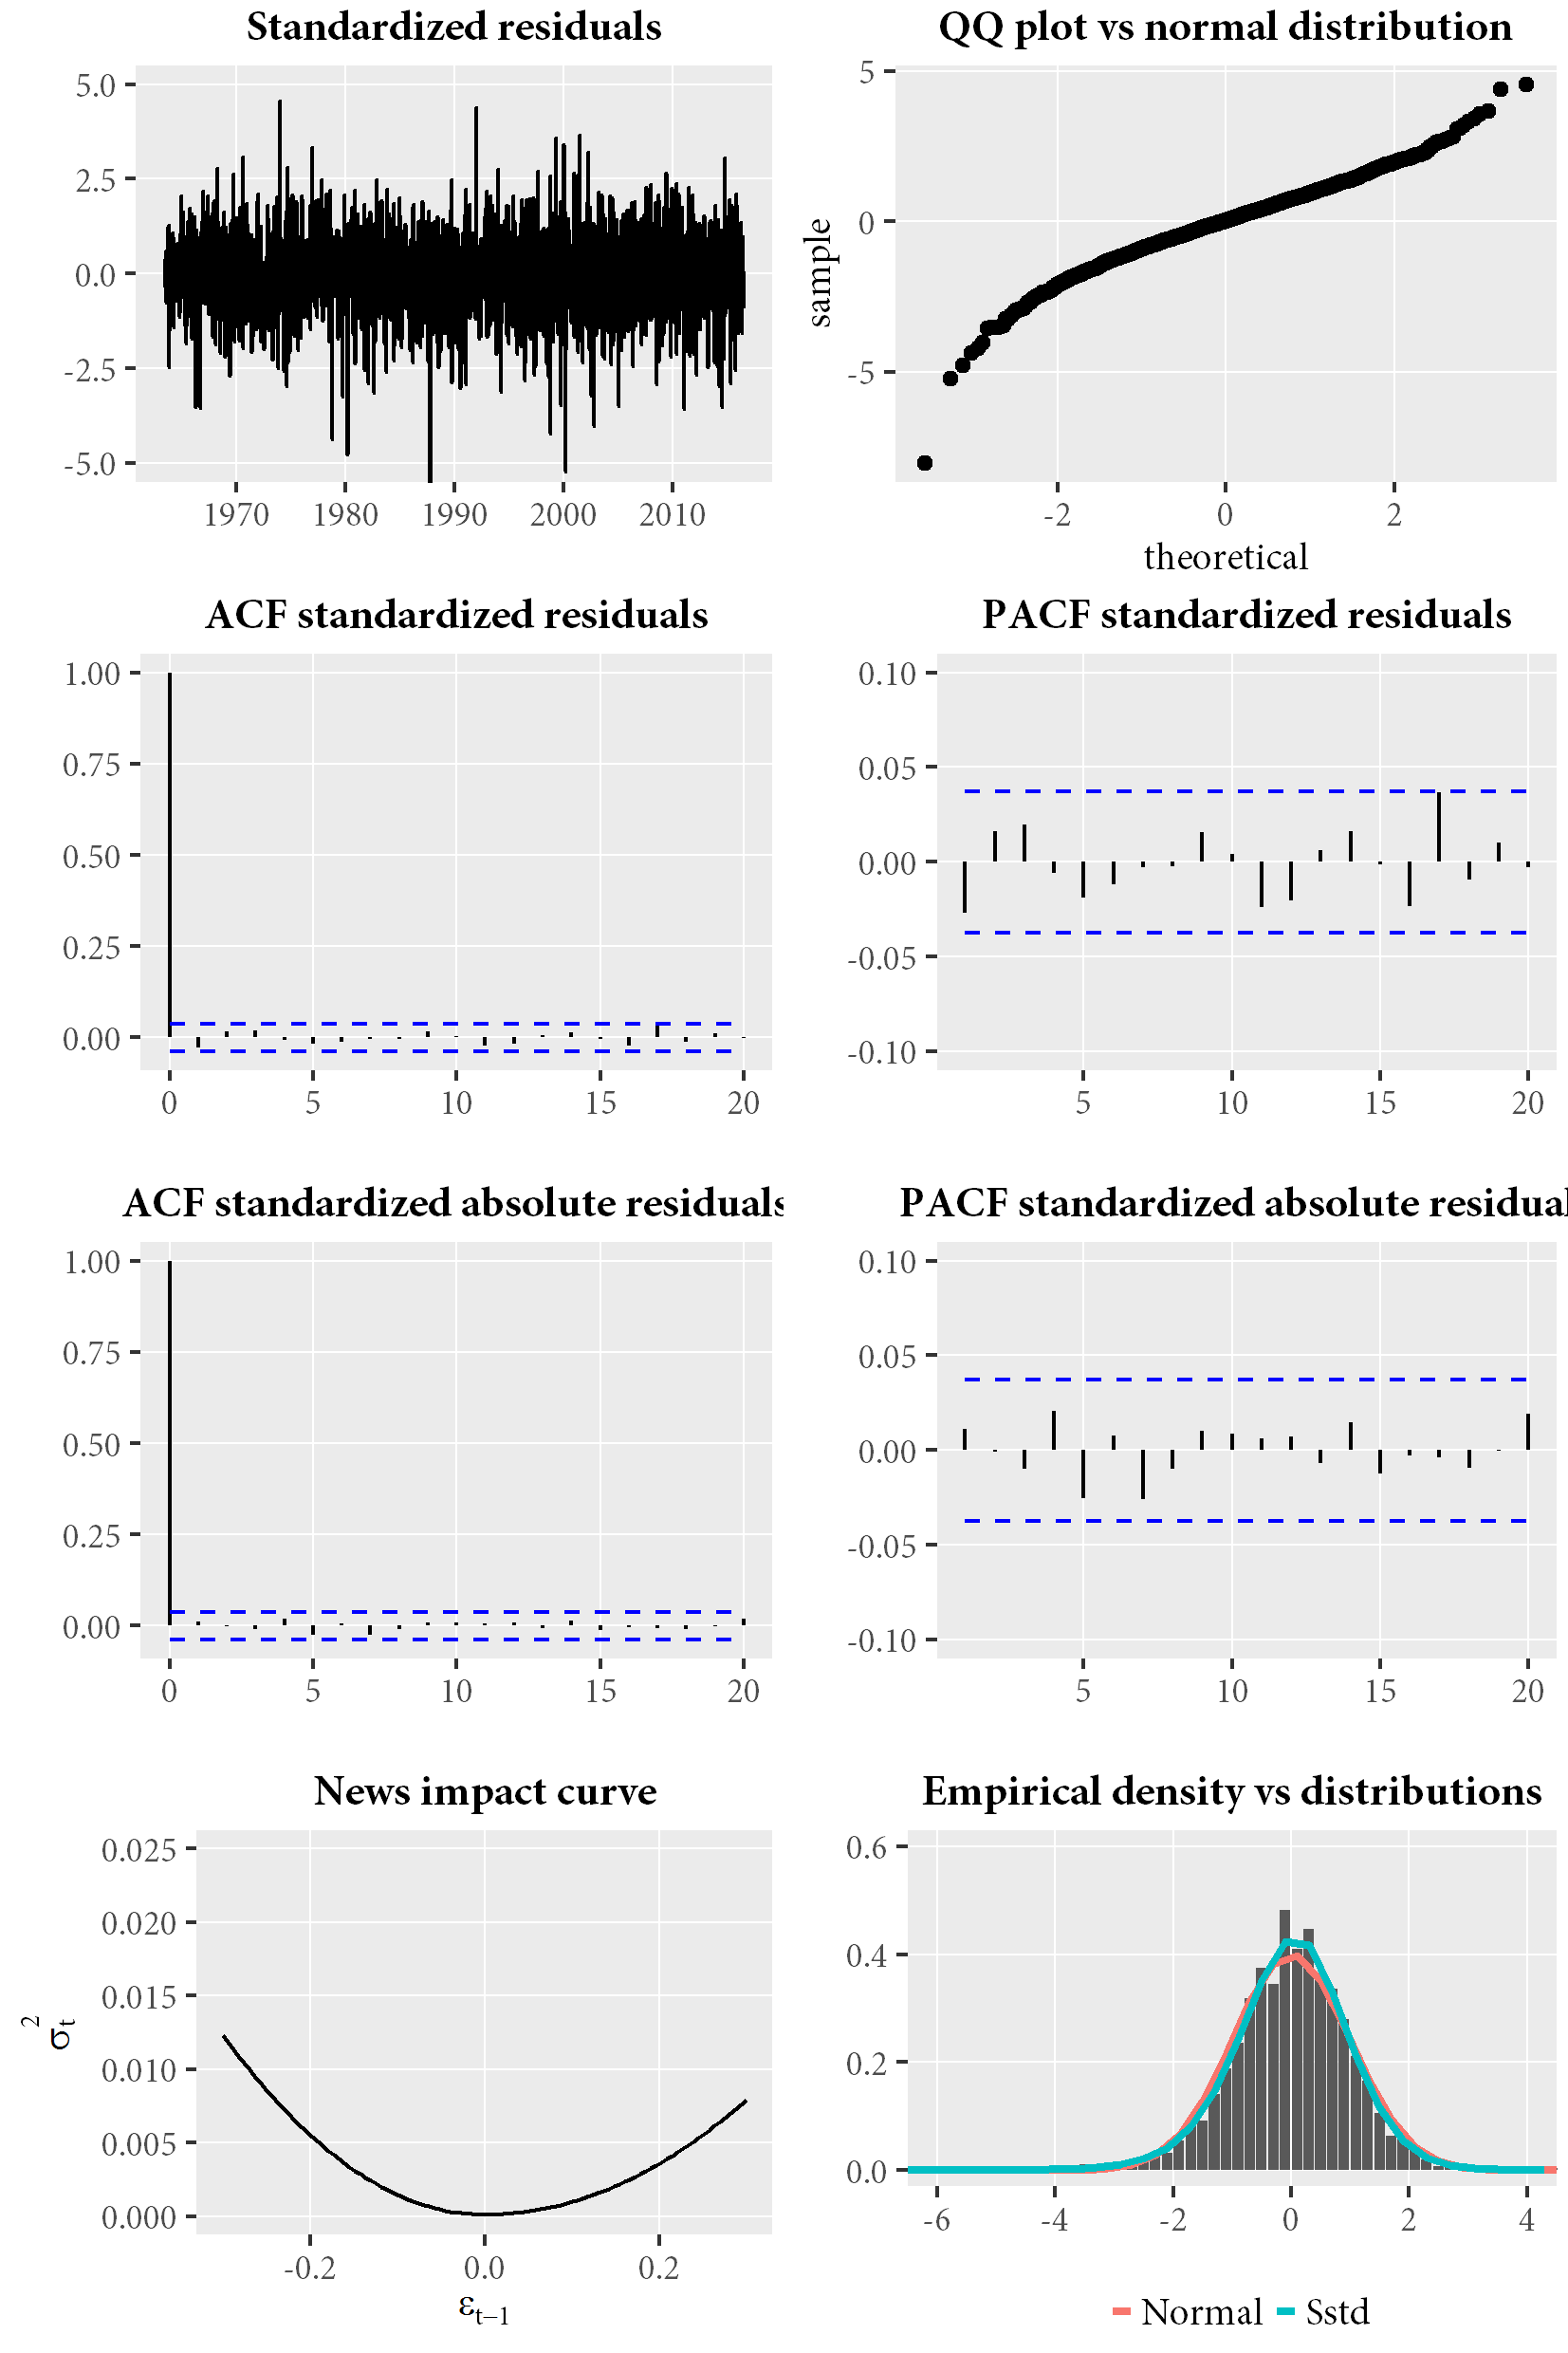
\includegraphics[scale=1]{graphics/garch/garch_diagnosticsSMB.png}  
  \bottomrule
  \vspace{3mm}
  \footnotesize
  We report diagnostics plots for the ARMA-GJR-GARCH residuals. Autocorrelation and partial autocorrelation functions are plotted with 95\% confidence bounds.
  \end{minipage}
\end{figure}
\begin{figure}[H]
  \caption{GARCH diagnostics plots - Mom}
  \label{diag:garchdiagMom}
  \toprule
  \centering
  \begin{minipage}{\textwidth}
  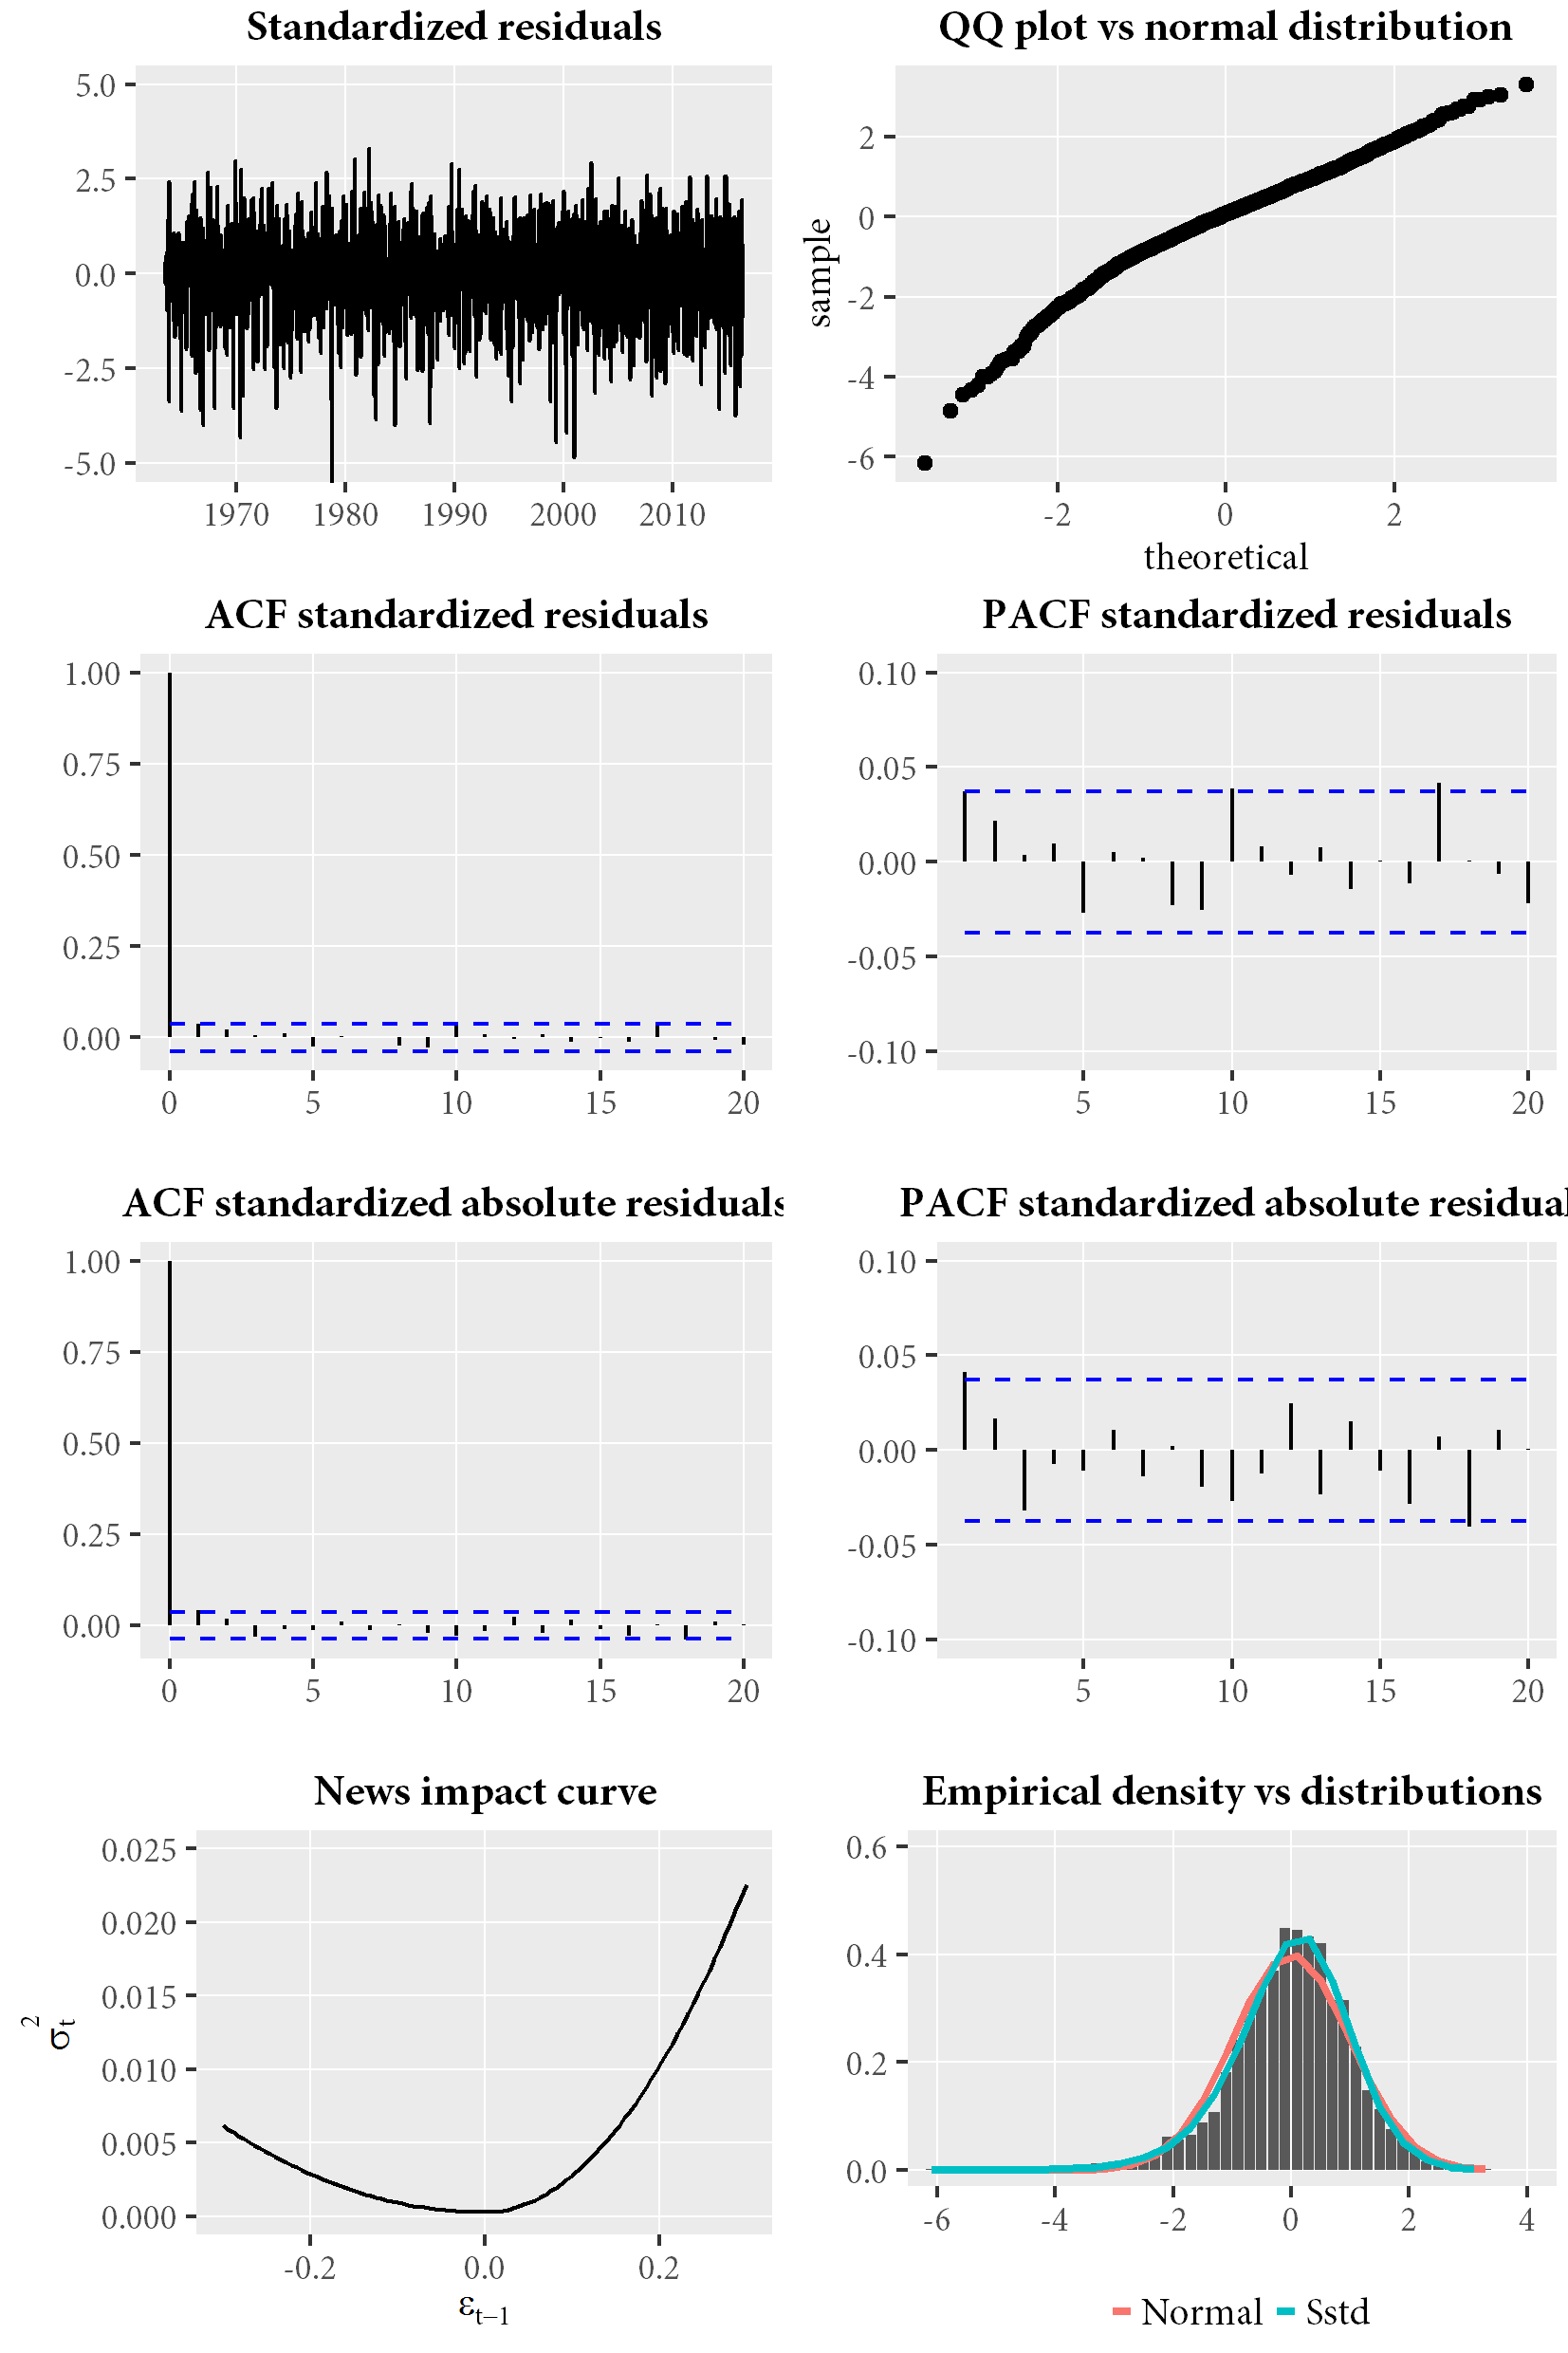
\includegraphics[scale=1]{graphics/garch/garch_diagnosticsMom.png}  
  \bottomrule
  \vspace{3mm}
  \footnotesize
  We report diagnostics plots for the ARMA-GJR-GARCH residuals. Autocorrelation and partial autocorrelation functions are plotted with 95\% confidence bounds.
  \end{minipage}
\end{figure}
\begin{figure}[H]
  \caption{GARCH diagnostics plots - RMW}
  \label{diag:garchdiagRMW}
  \toprule
  \centering
  \begin{minipage}{\textwidth}
  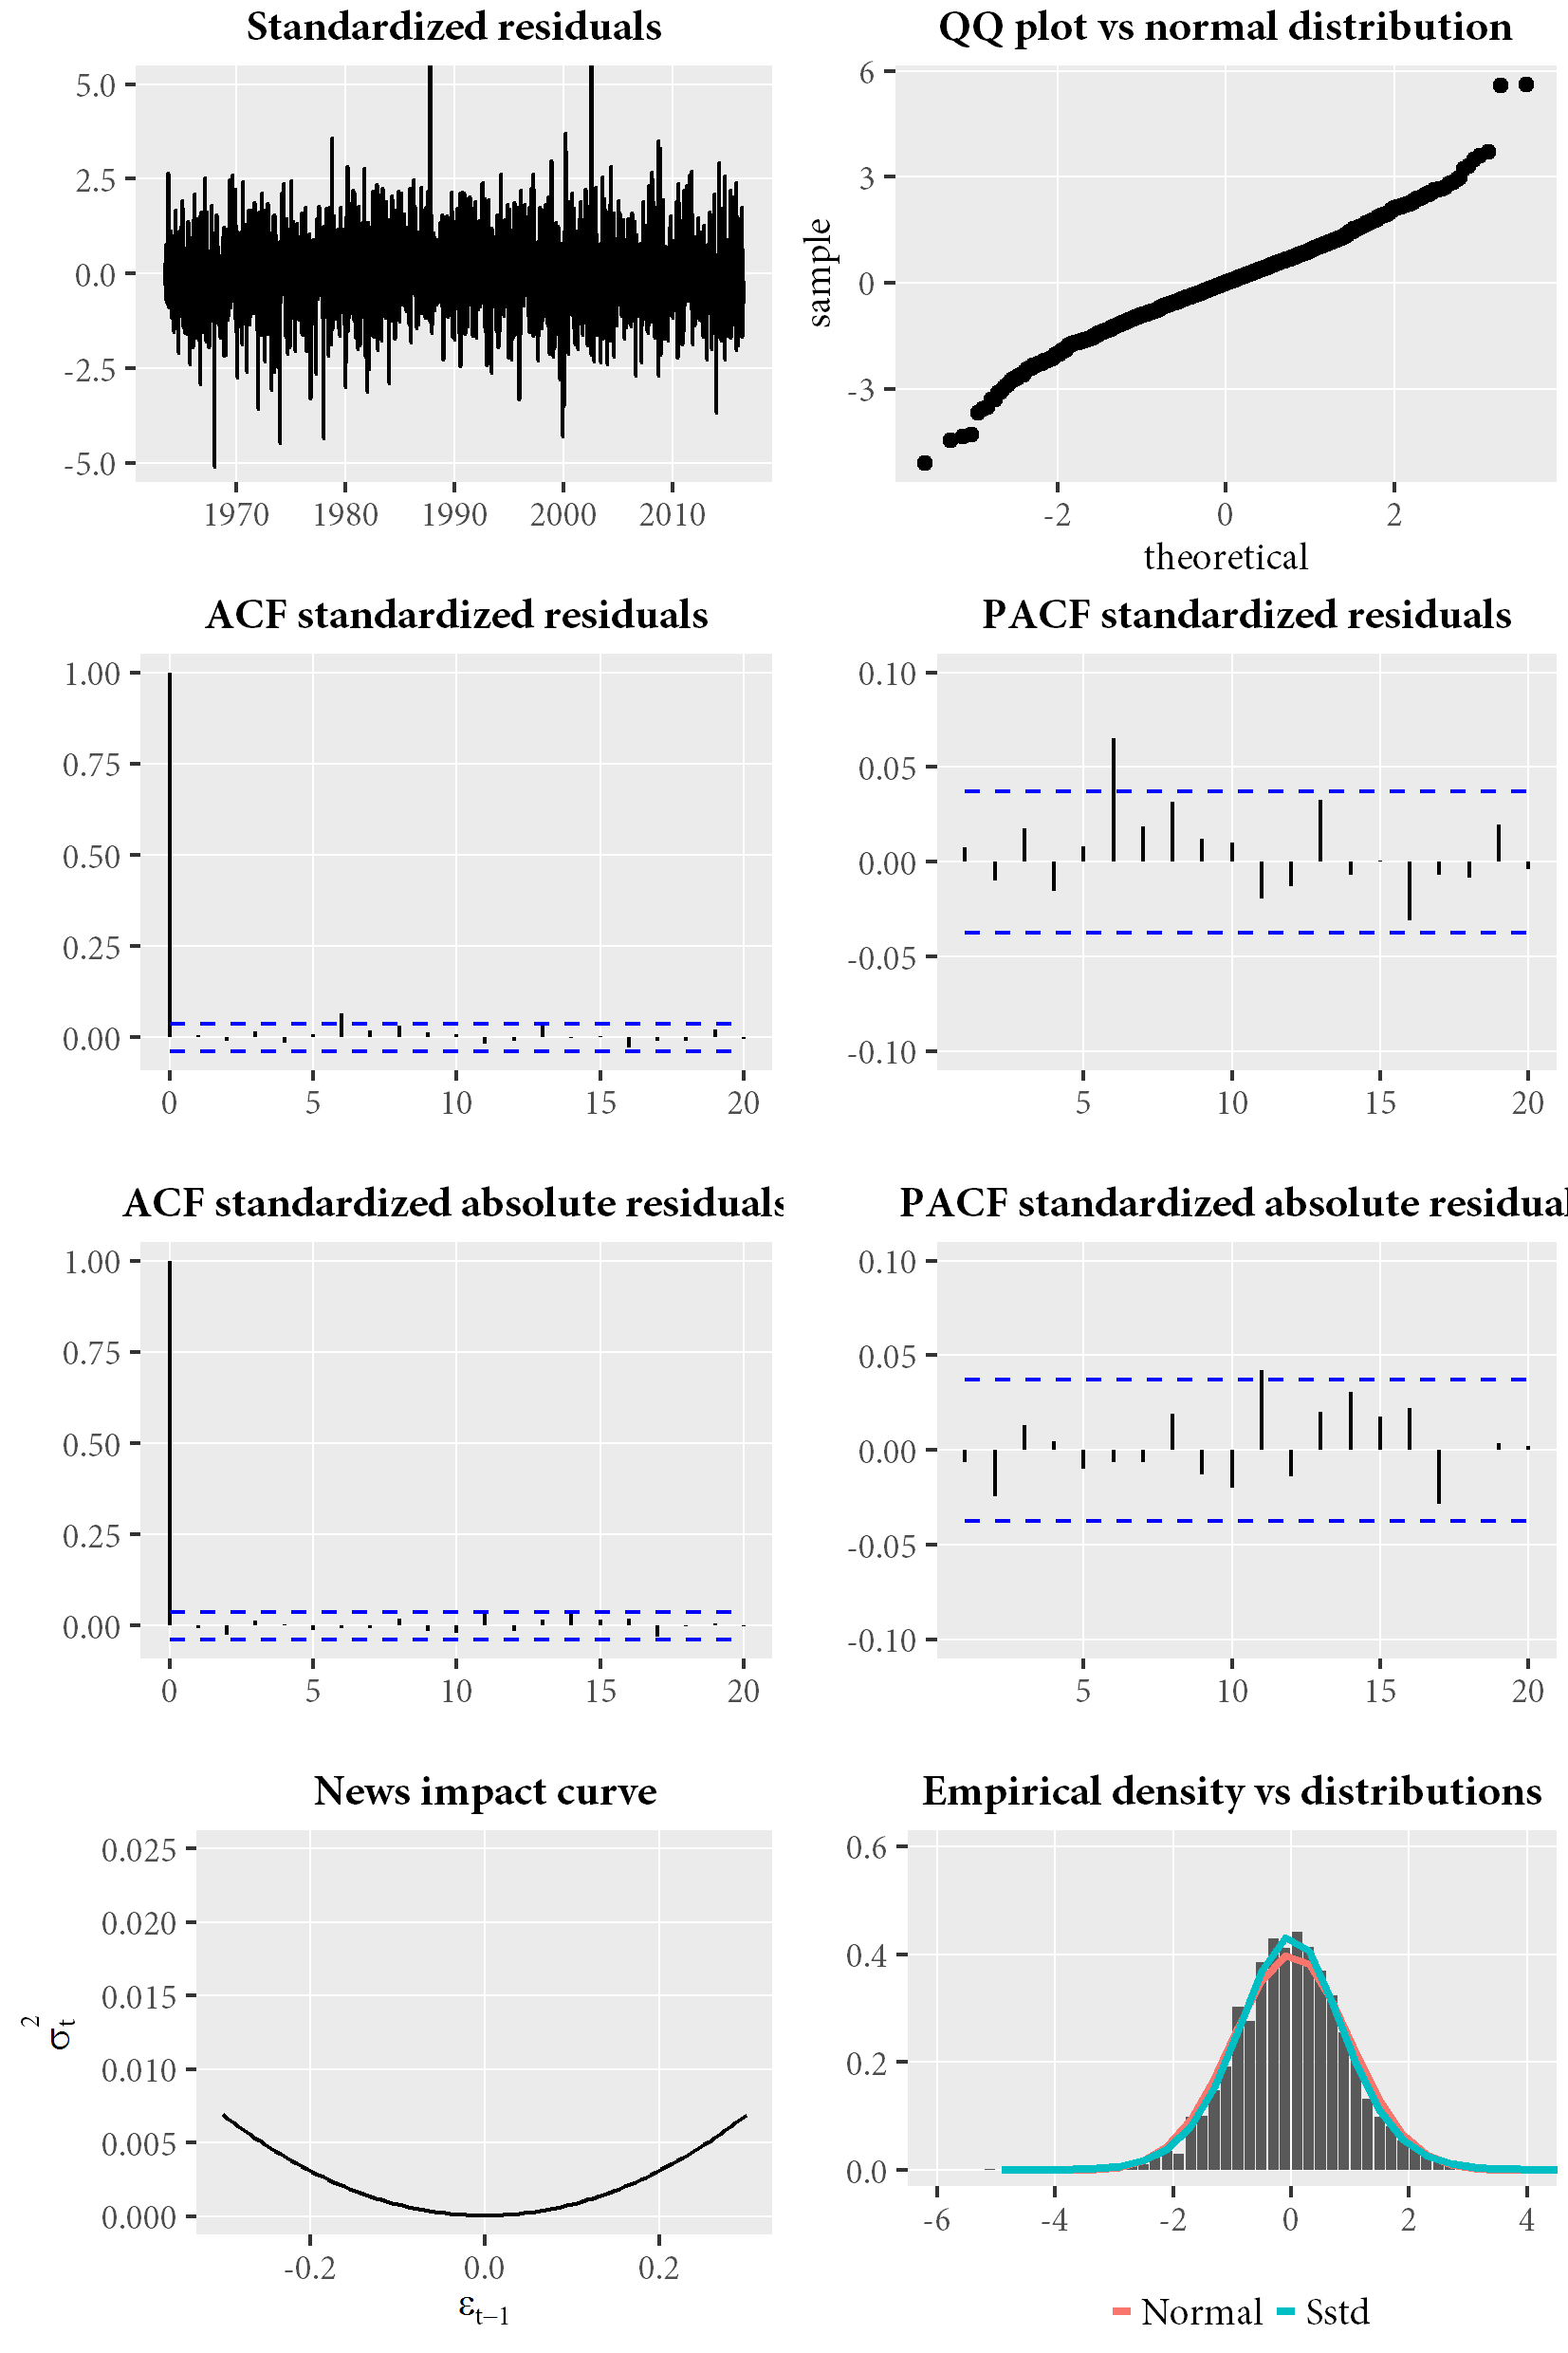
\includegraphics[scale=1]{graphics/garch/garch_diagnosticsRMW.png}  
  \bottomrule
  \vspace{3mm}
  \footnotesize
  We report diagnostics plots for the ARMA-GJR-GARCH residuals. Autocorrelation and partial autocorrelation functions are plotted with 95\% confidence bounds.
  \end{minipage}
\end{figure}
\begin{figure}[H]
  \caption{GARCH diagnostics plots - CMA}
  \label{diag:garchdiagCMA}
  \toprule
  \centering
  \begin{minipage}{\textwidth}
  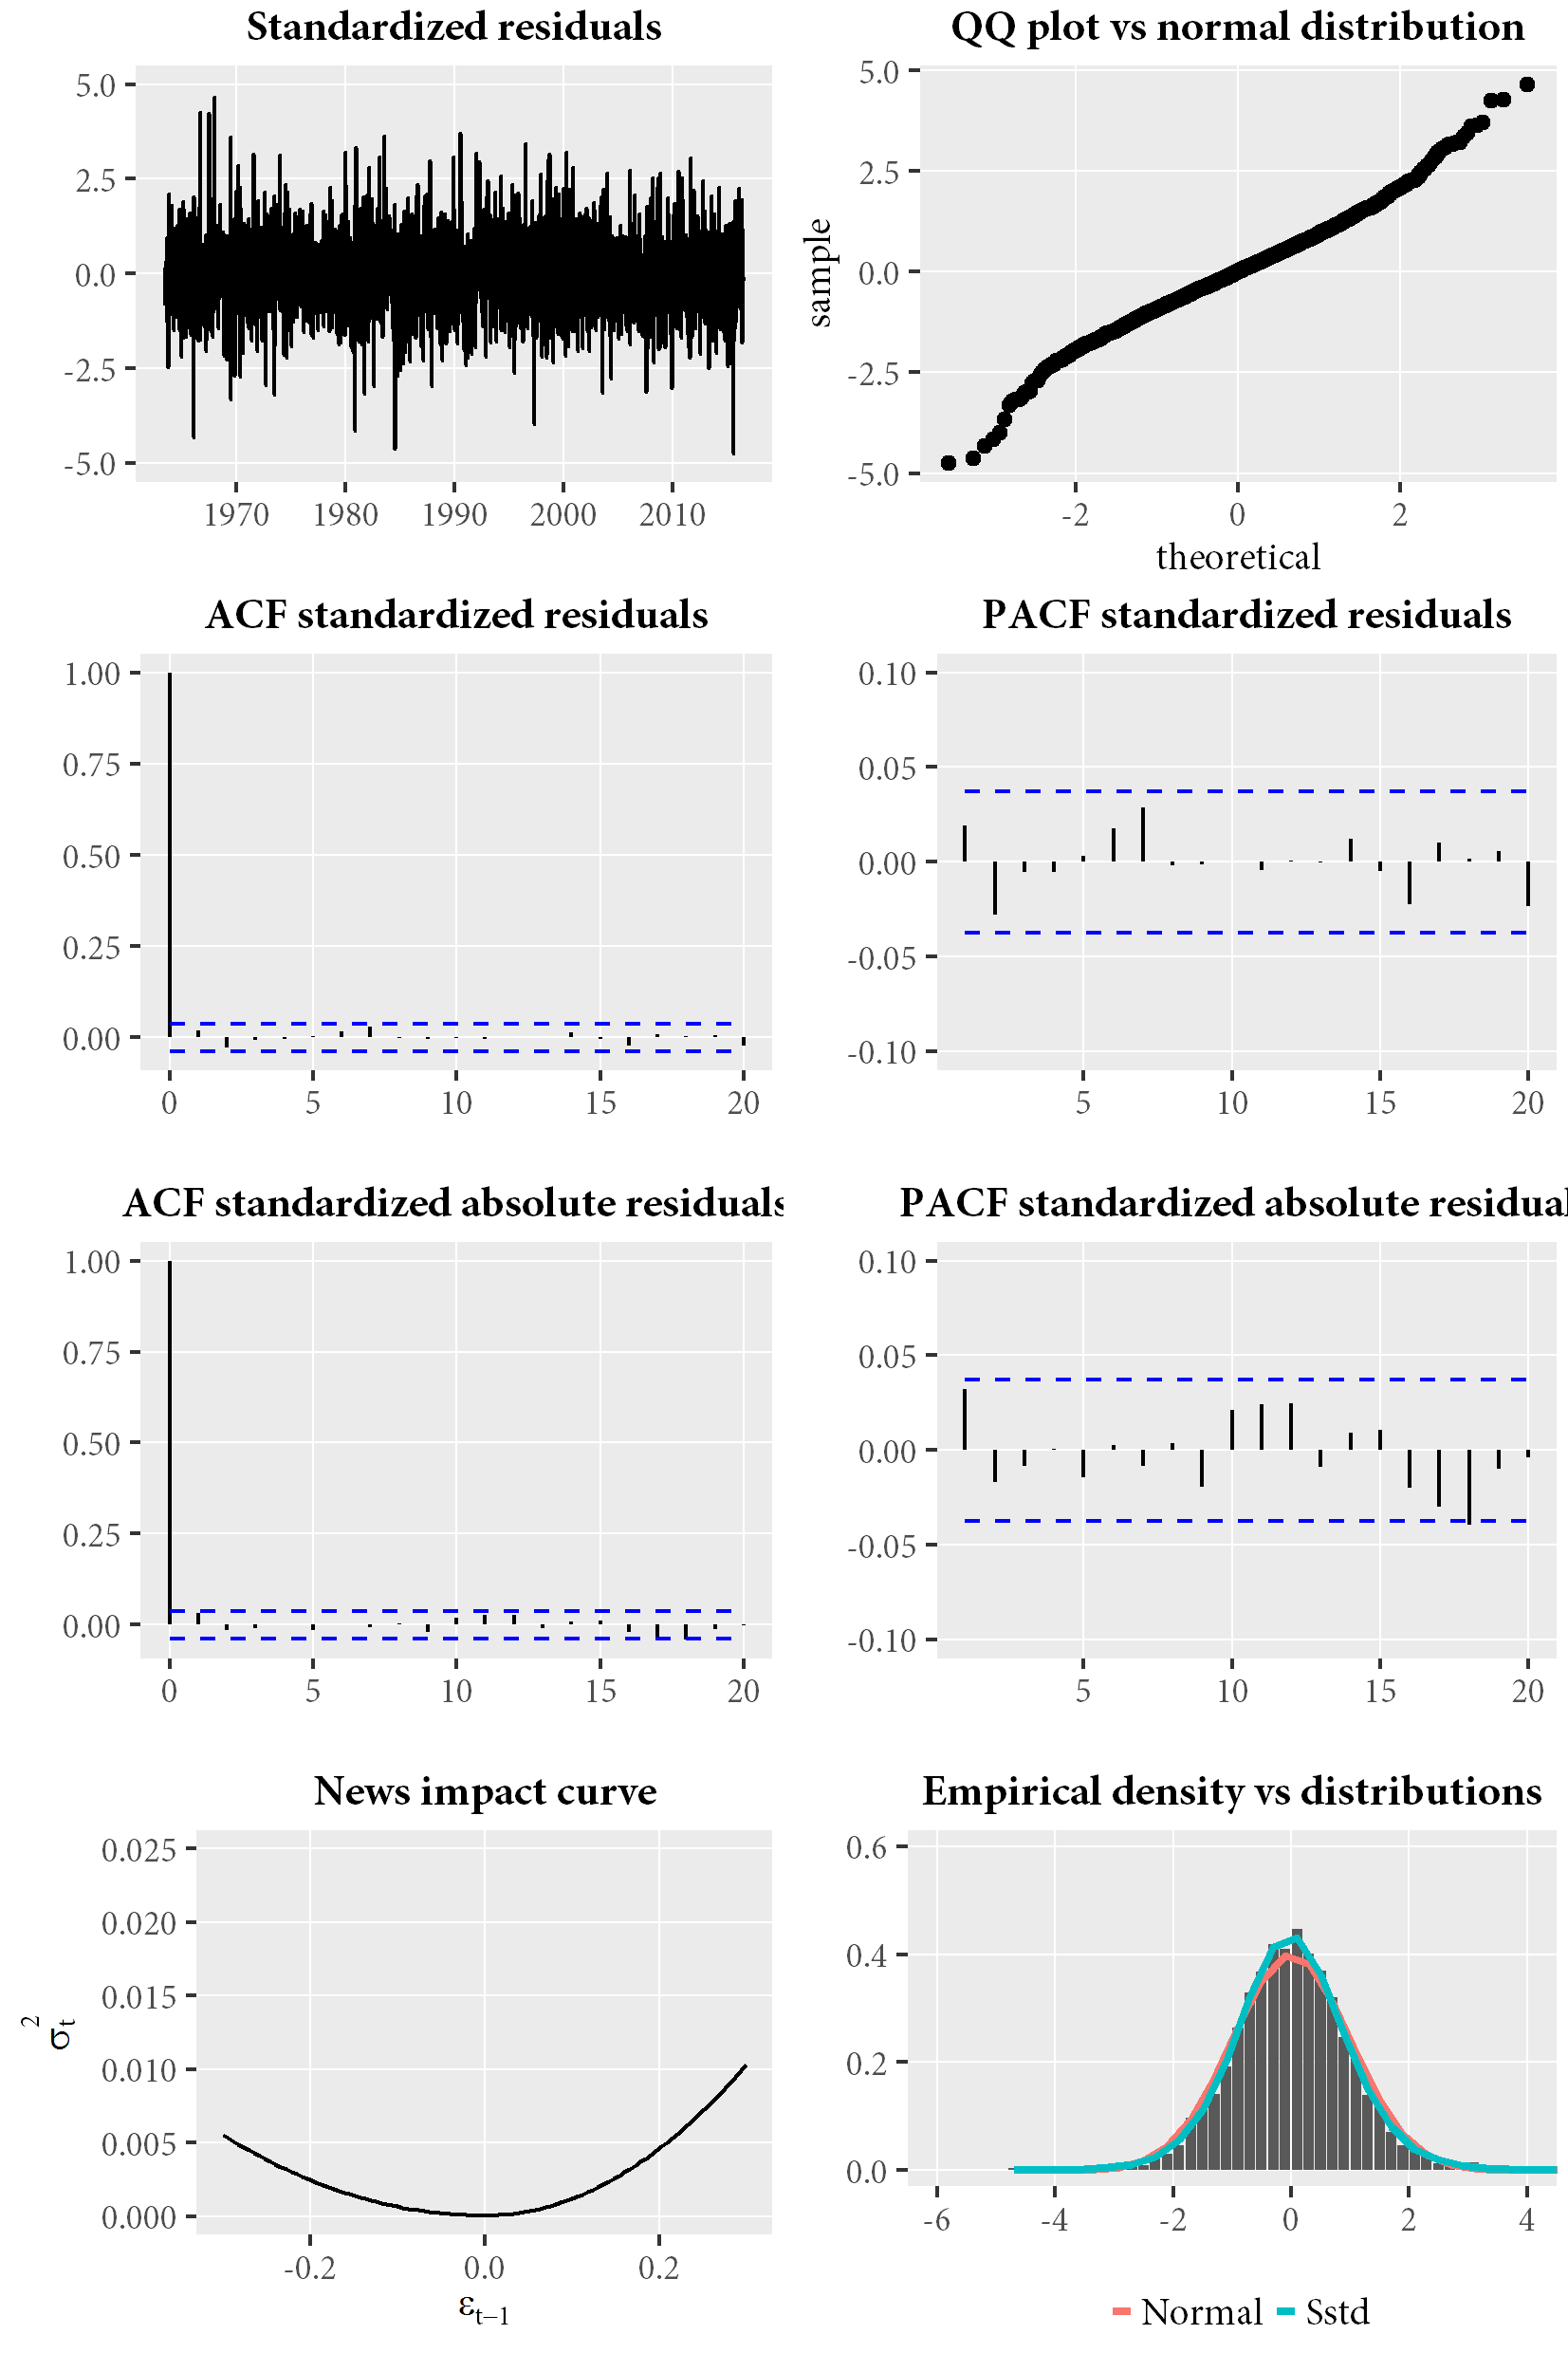
\includegraphics[scale=1]{graphics/garch/garch_diagnosticsCMA.png}  
  \bottomrule
  \vspace{3mm}
  \footnotesize
  We report diagnostics plots for the ARMA-GJR-GARCH residuals. Autocorrelation and partial autocorrelation functions are plotted with 95\% confidence bounds.
  \end{minipage}
\end{figure}